%!TEX root=./pfc.tex
\chapter[Funcionamiento]{\label{}
Funcionamiento}

El primer paso que debe realizar el usuario será cargar la página principal de Moodle, en la que se ofrecerán todos los cursos disponibles. Para ello, deberá escribir en la barra de dirección del navegador la siguiente línea: http://"direcciónHost":"puertoComunicación" / "nombreServidor". En \emph{"direcciónHost"}, como su mismo nombre indica, habrá que escribir la dirección del host al que el usuario debe conectarse. En \emph{"puertoComunicación"} habrá que escribir el puerto de comunicación por el cual se comunica con el host especificado anteriormente. En \emph{"nombreServidor"} habrá que escribir la dirección y el nombre asociados con el servidor de Moodle.

Una vez cargada esta pantalla principal, se le presentará al usuario una imagen como la siguiente:

\begin{figure}[h]
	\label{pantallaprincipal.eps}
	\includegraphics[width=\textwidth]{./img/pantallaprincipal.eps}
	\caption{Pantalla principal de Moodle con todos los cursos disponibles}
\end{figure}

Ahora el usuario deberá elegir el curso donde está matriculado, y una vez hecho esto entrar al sistema indicando su nombre de usuario y contraseña.

Para ello en primer lugar vamos a seleccionar el curso haciendo click sobre él:

\begin{figure}[h]
	\label{pantallaprincipalselect.eps}
	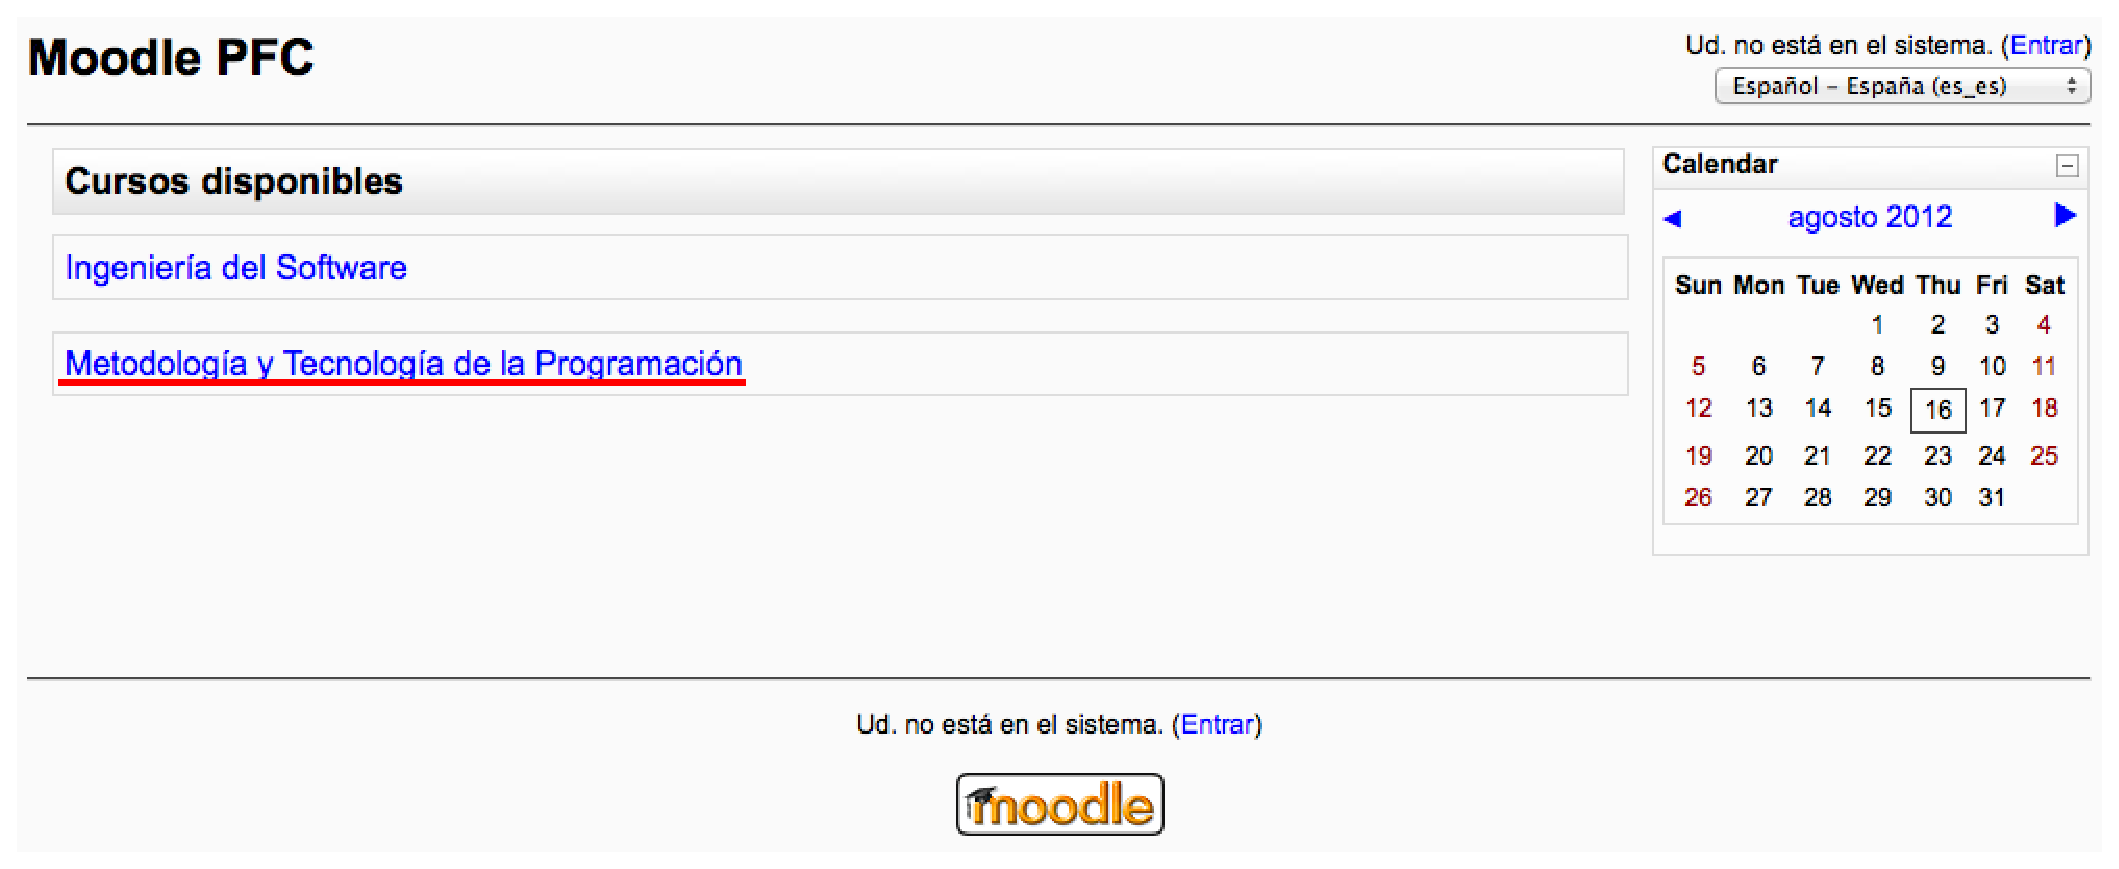
\includegraphics[width=\textwidth]{./img/pantallaprincipalselect.eps}
	\caption{Selección del curso}
\end{figure}

Y posteriormente nos autentificamos en él:

\begin{figure}[h]
	\label{login.eps}
	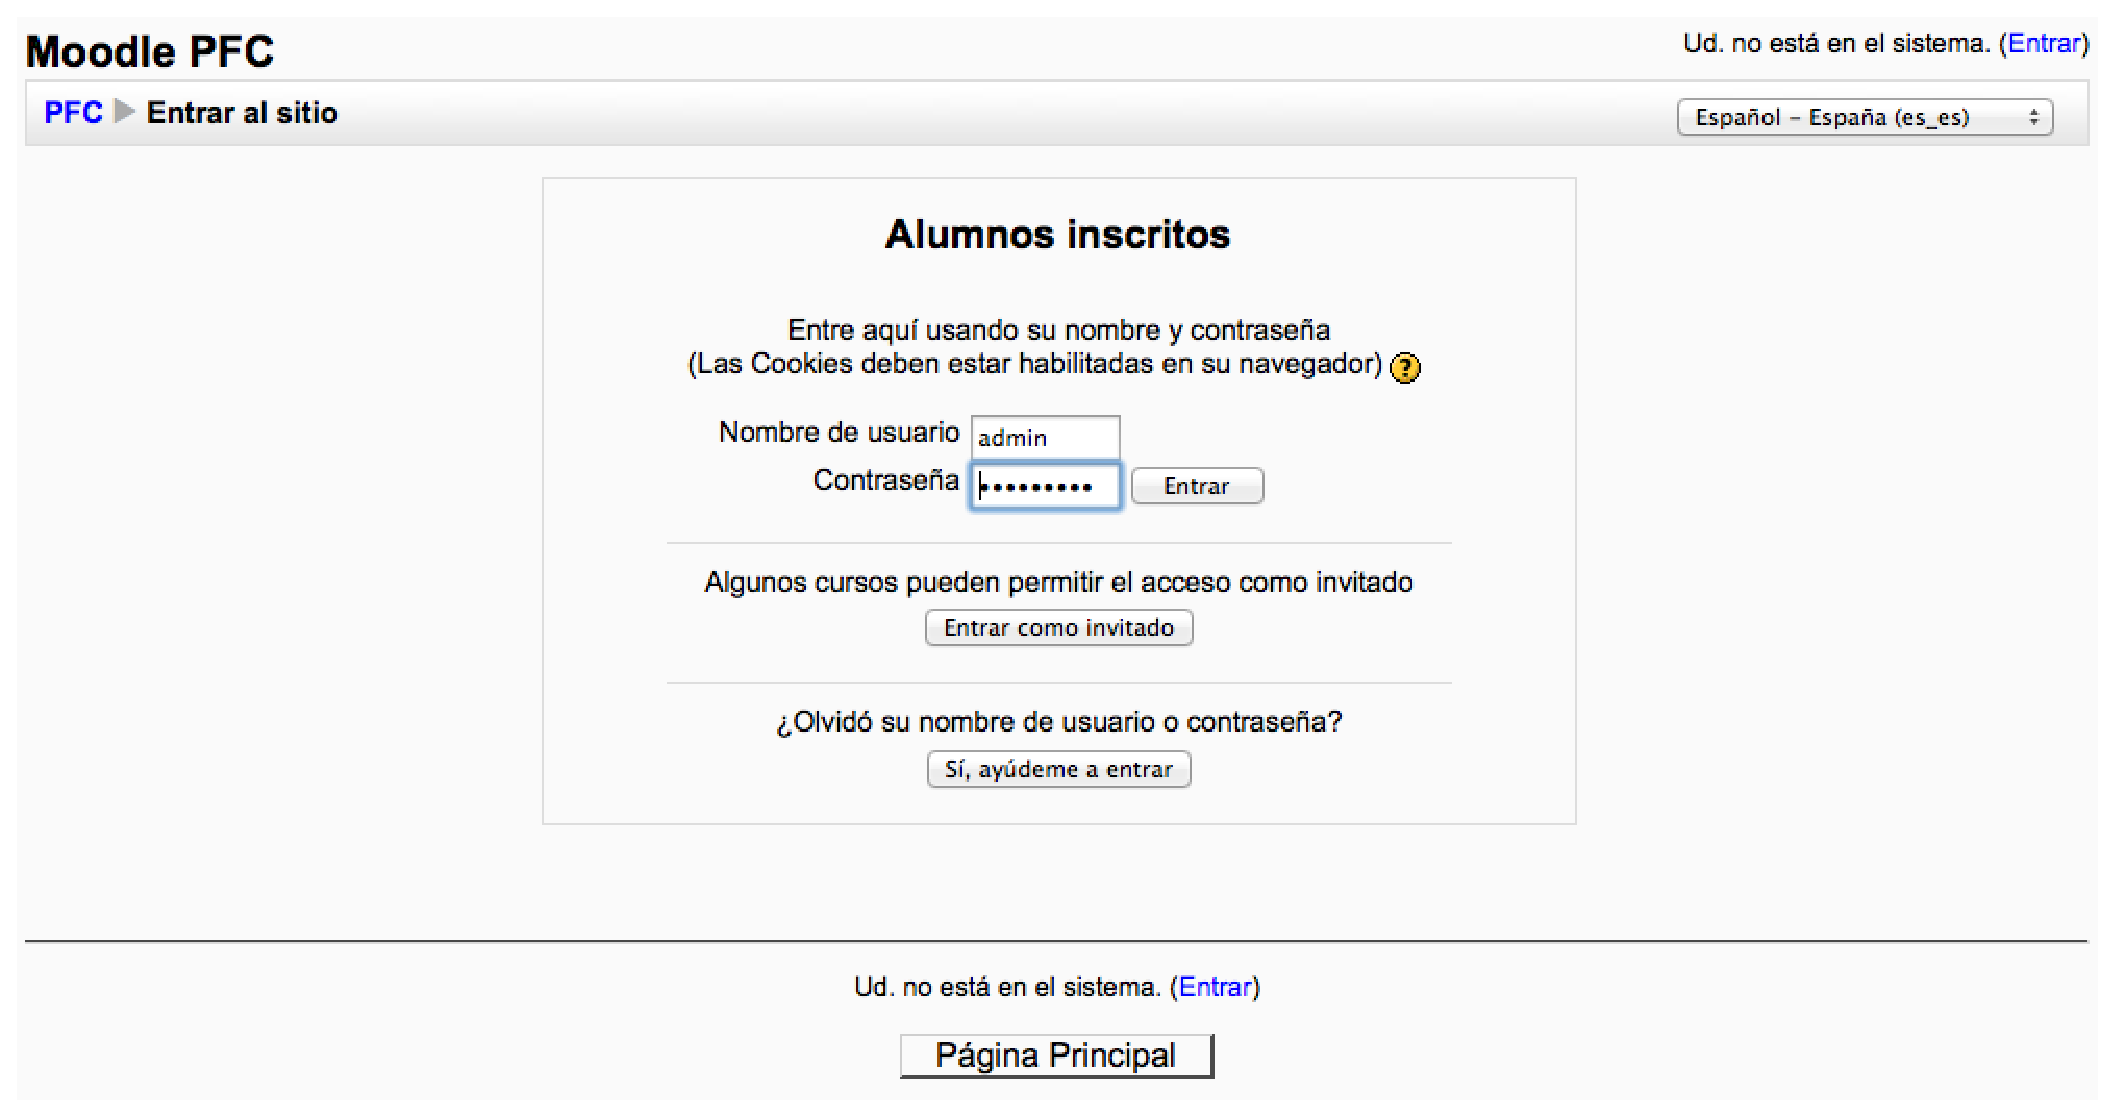
\includegraphics[width=\textwidth]{./img/login.eps}
	\caption{Pantalla de login}
\end{figure}

\newpage

Si la autentificación tiene éxito, se le mostrará al usuario todo el contenido del curso. A su vez, si dicho usuario tiene privilegios de edición sobre el curso podrá añadir una nueva \emph{wikicode} a los contenidos del curso.

\begin{figure}[h]
	\label{addwikicode.eps}
	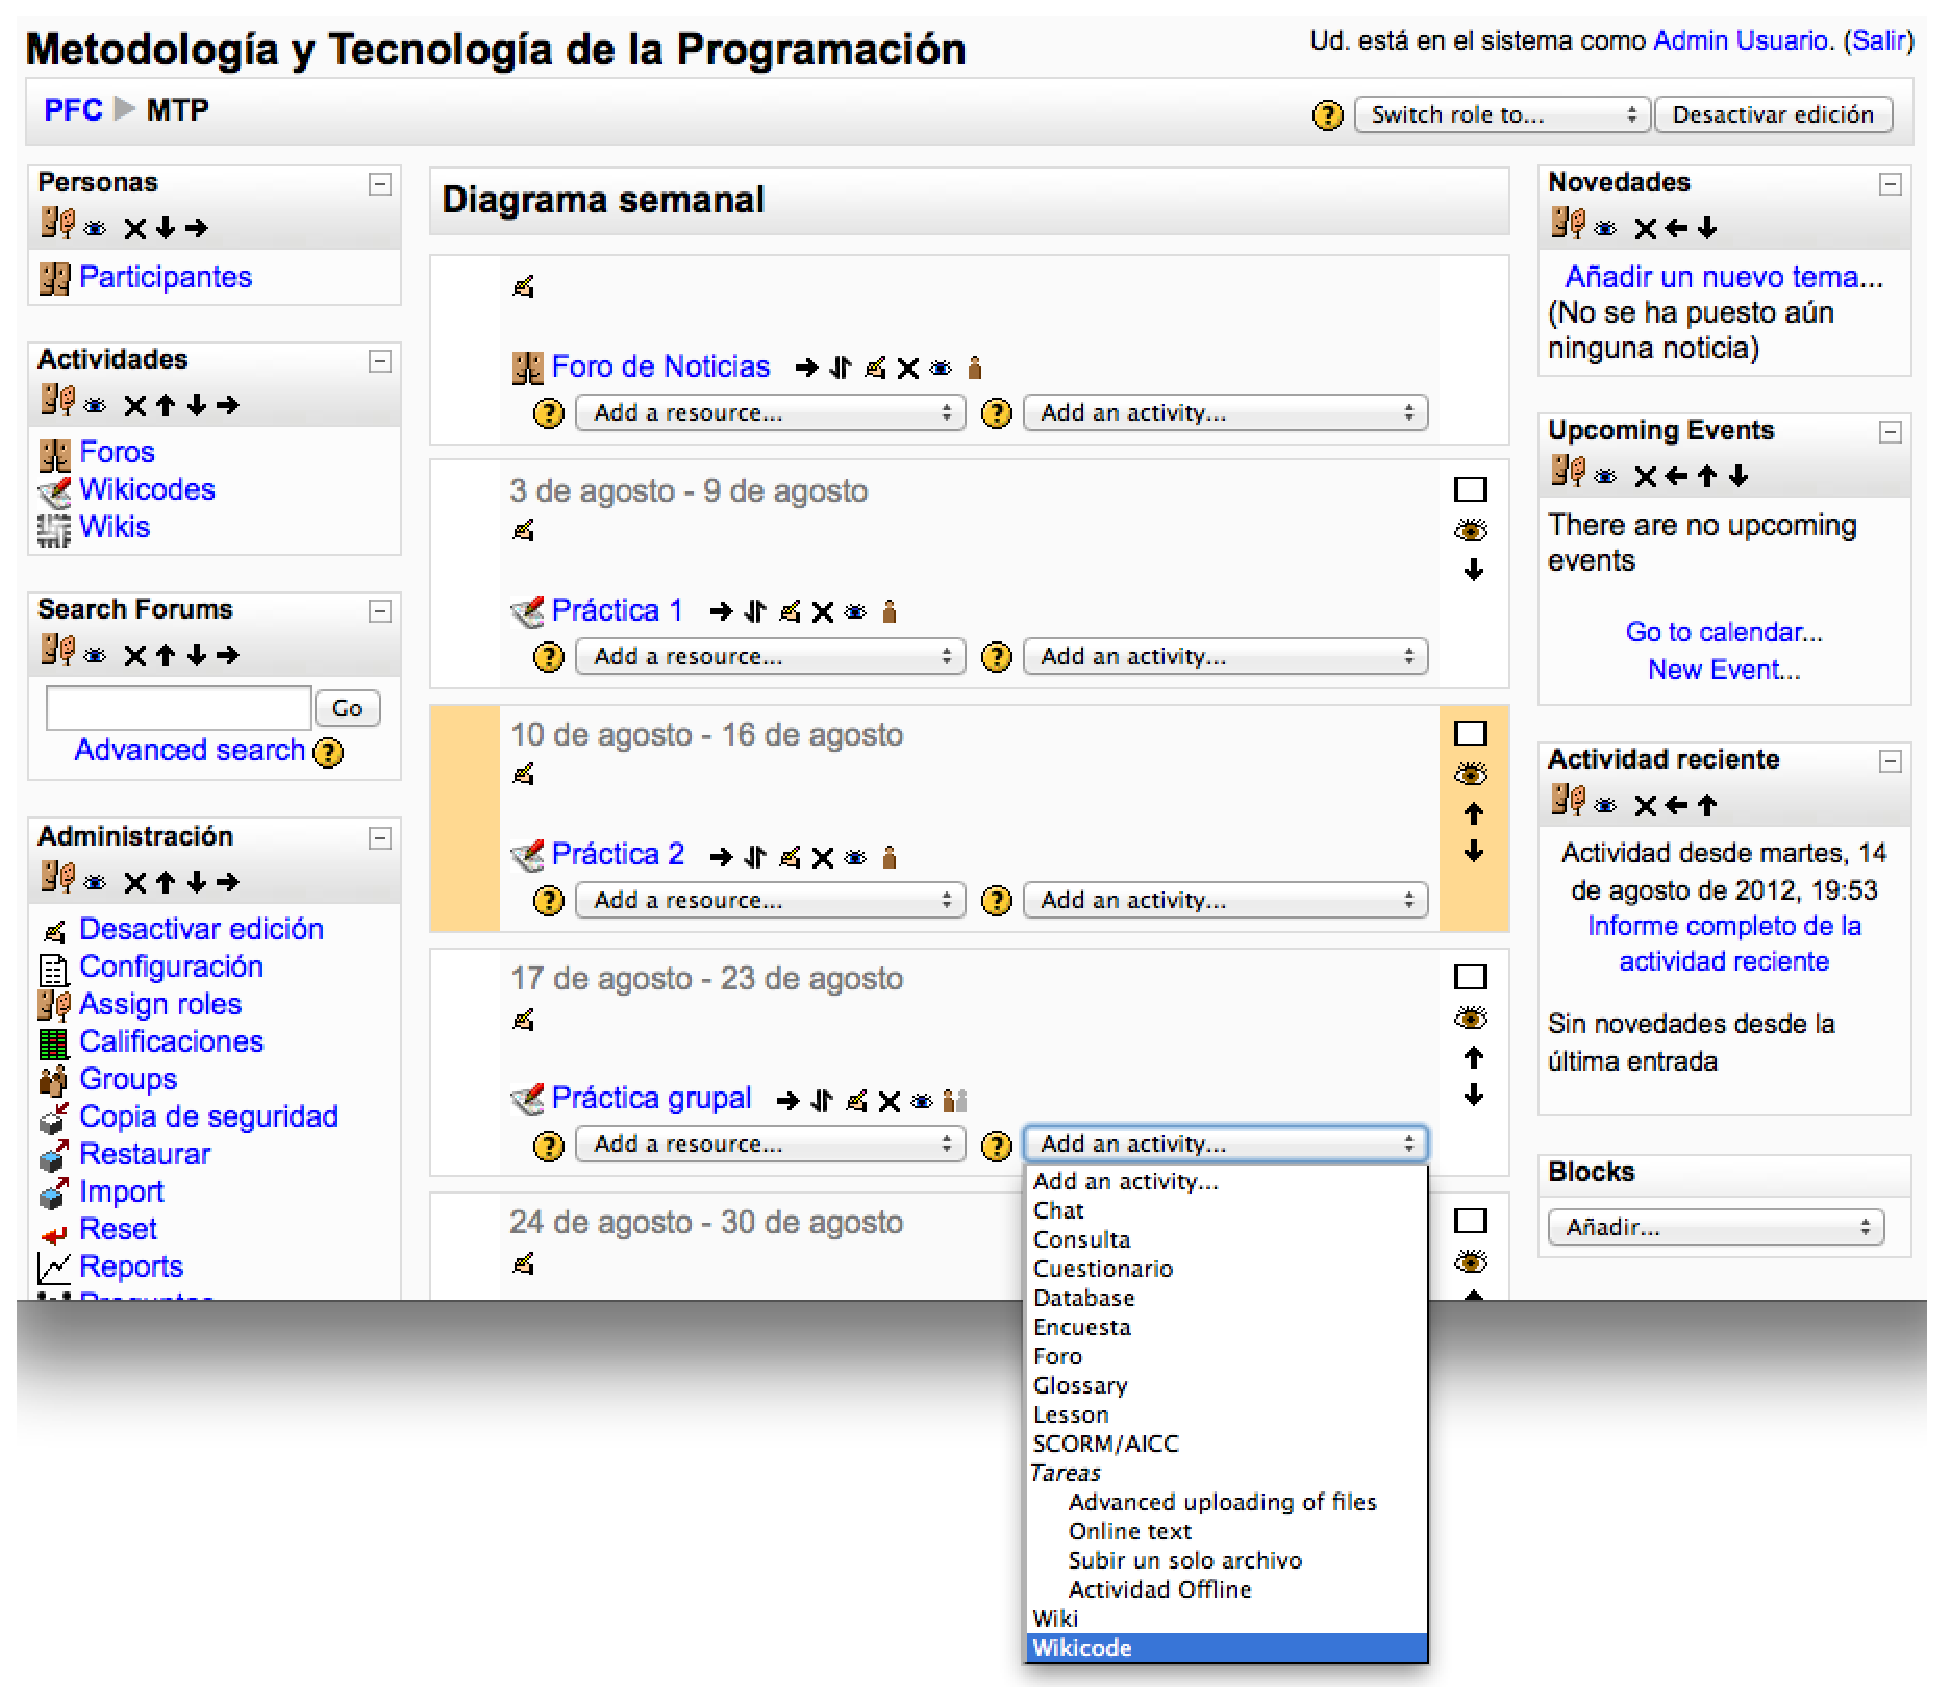
\includegraphics[width=\textwidth]{./img/addwikicode.eps}
	\caption{Añadimos una Wiki de edición de código al curso}
\end{figure}

\newpage

Una vez que se cree un nuevo módulo \emph{wikicode} para el curso Moodle seleccionado, nos aparecerá un formulario con todas las opciones para su configuración.

\begin{figure}[h]
	\label{v1create1.eps}
	\includegraphics[width=\textwidth]{./img/v1create1.eps}
	\caption{Pantalla de Configuración de una nueva Wikicode}
\end{figure}

Los parámetros que se van a configurar son los siguientes:

\begin{description}
	\item[Wiki Name:] Obligatorio. Nombre que asignamos a nuestra Wiki para identificar en la pantalla principal del curso.
	\item[First Page Name:] Obligatorio. Nombre interno que define a nuestro código.
	\item[Unix Compiler Path:] Obligatorio. Ruta hacia el compilador con el que queremos que se compilen los ejecutables para OS basados en Unix.
	\item[Windows Compiler Path:] Obligatorio. Ruta hacia el compilador con el que queremos que se compilen los ejecutables para Windows.
	\item[Wiki Mode:] Colaborativa o Individual. Como su nombre indica nos dice el modo en que actuará la Wiki.
	\item[Default Format:] Es el formato del editor. La única opción actualmente es WCode, que es sobre la que trabaja nuestro editor. En el futuro se puede ampliar a más formatos.
	\item[Force Format:] Check que nos impide cambiar el formato de una Wiki una vez creada.
	\item[Group Mode:] Tres opciones:
	\begin{description}
		\item[No groups:] No hay subgrupos. Cada usuario es miembro de una gran comunidad.
		\item[Separate Groups:] Cada grupo solo puede ver su propia Wiki, las wikis de otros grupos son invisibles para él.
		\item[Visible Groups:] Un usuario sólo puede modificar la Wiki de su grupo, pero el resto de Wikis son visibles para él.
	\end{description}
	\item[Visible:] Indica si la Wiki es visible.
	\item[ID Number:] Si está vacía el sistema asignará un ID por nosotros. Si lo rellenamos podemos forzar el ID.
	\item[Grade category:] Actualmente sólo dispone de la categoría \emph{Uncategorised}, pero si se desea en un futuro se pueden crear categorías y agrupar Wikis en ellas.
\end{description}

\newpage

Una vez creada podemos volver al curso o entrar a la Wiki. De todos modos, aunque posterguemos esta entrada, en la primera visita nos preguntará para confirmar los cambios. 

\vspace{2cm}

\begin{figure}[h]
	\label{v1create2.eps}
	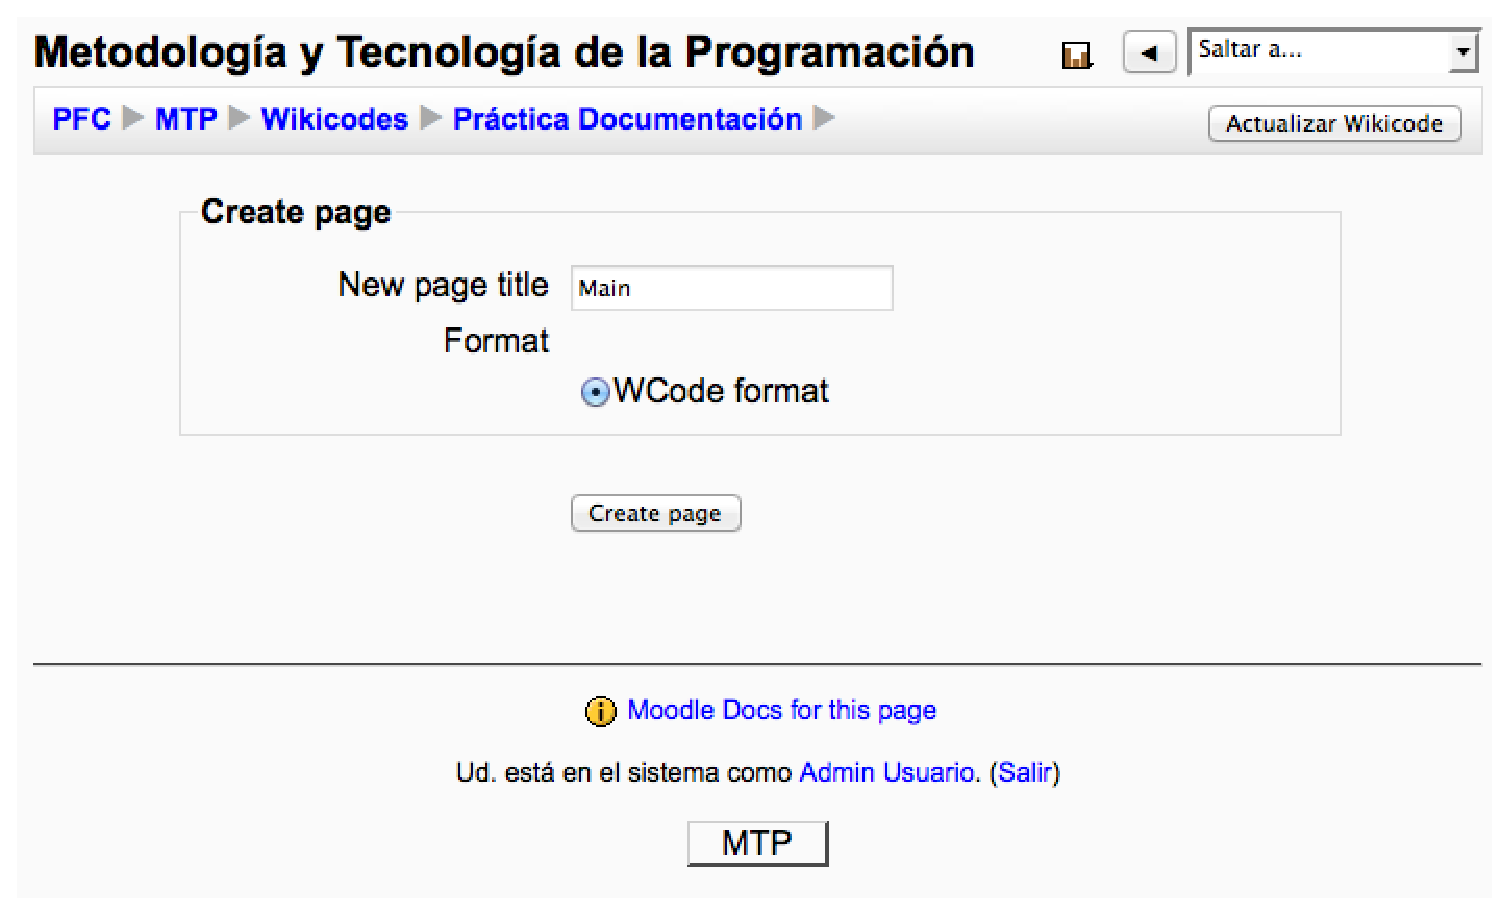
\includegraphics[width=\textwidth]{./img/v1create2.eps}
	\caption{Pantalla de confirmación de parámetros Wikicode}
\end{figure}

También hay que hacer ver, que siempre que nos encontremos en una pantalla de Wikicode, en la esquina superior derecha tendremos un botón de \emph{Actualizar Wikicode} donde podremos variar una gran cantidad de parámetros.

\newpage

Una vez se haya creado dicha Wikicode, lo primero que nos aparecerá será la pantalla de edición.

\begin{figure}[h]
	\label{v1edit1.eps}
	\includegraphics[width=\textwidth]{./img/v1edit1.eps}
	\caption{Editor de Código Colaborativo Wikicode}
\end{figure}

Sobre el editor (sección \ref{editSection}) hablaremos con mayor profundidad a partir en la página \pageref{editSection}.

Del mismo modo, si deseamos tener una mayor información sobre el código, será tan simple como pulsar el botón \emph{log} de la pestaña superior.

\begin{figure}[h]
	\label{v1log.eps}
	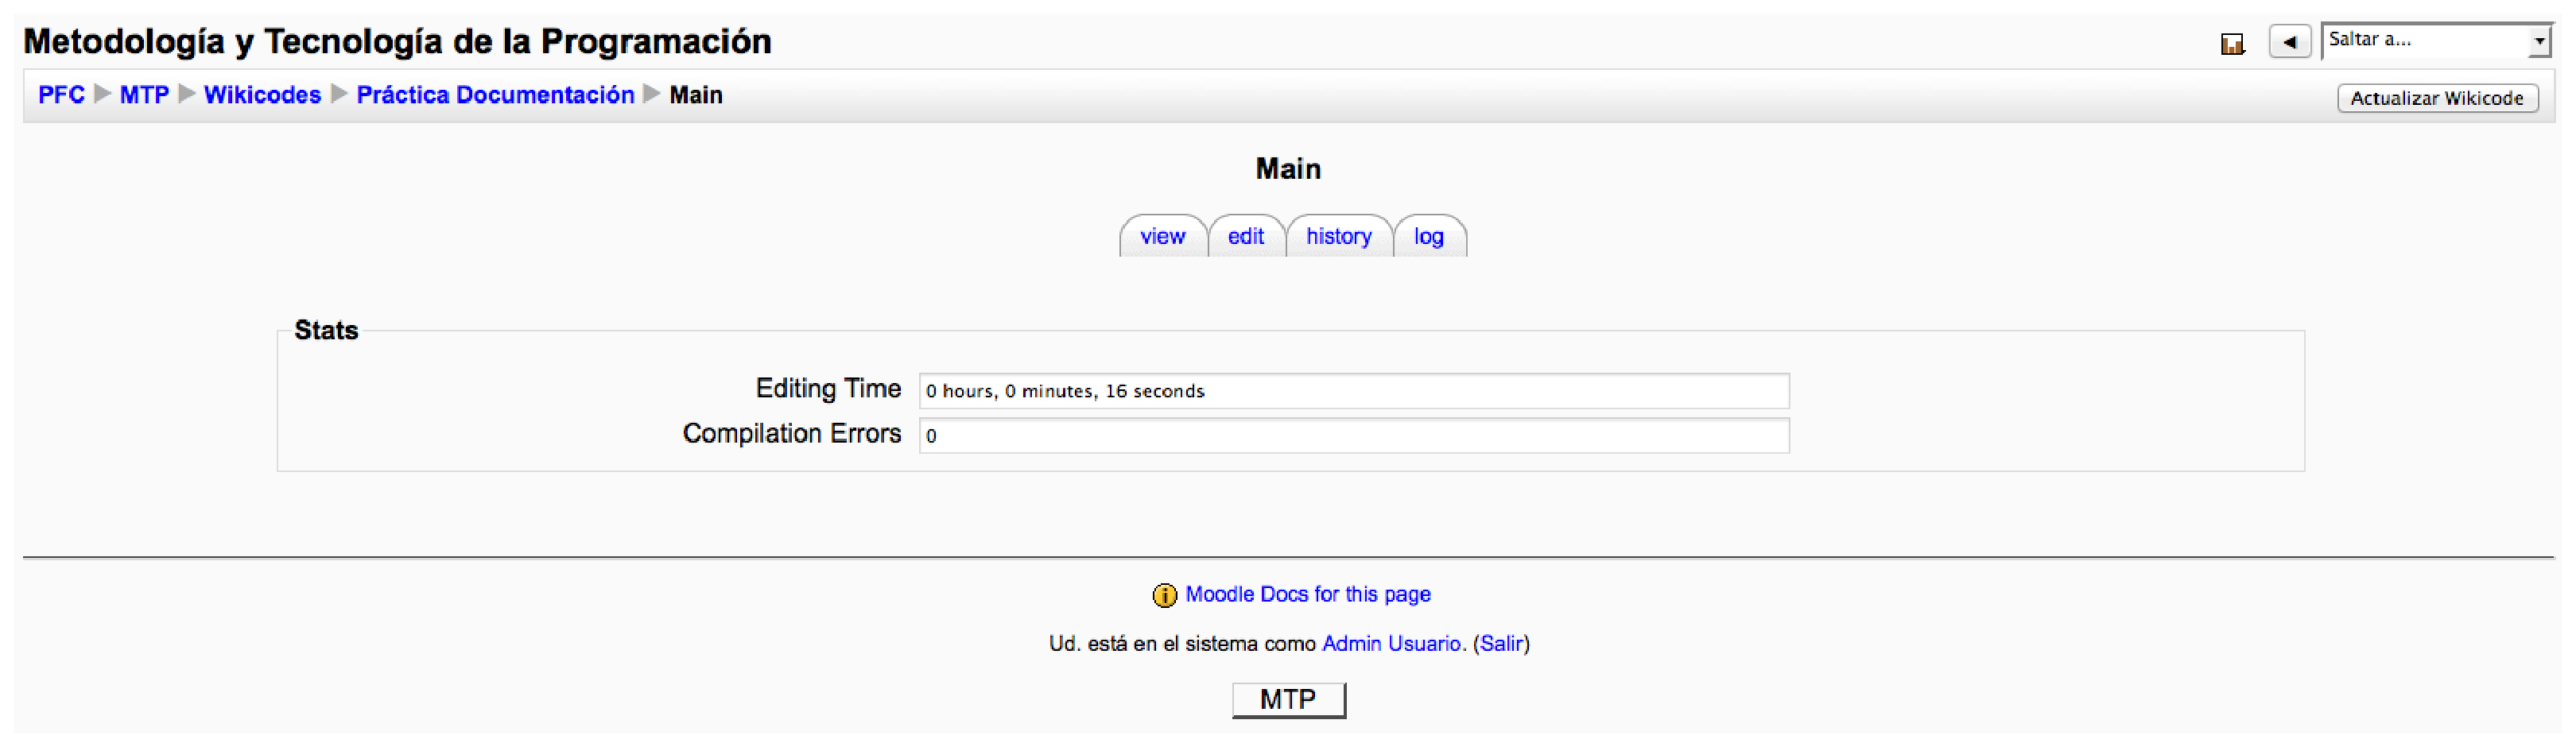
\includegraphics[width=\textwidth]{./img/v1log.eps}
	\caption{Log Wikicode}
\end{figure}

En él, como podemos comprobar, se nos informa del tiempo que se ha tardado en desarrollar el código y el número de errores de compilación que ha habido hasta el momento.

Las funcionalidades comentadas hasta el momento son comunes tanto de la versión \emph{1.x} de Moodle como de la \emph{2.x}. A partir de este momento vamos a diferenciar una serie de pantallas que son propias de cada versión.

\section{Funciones específicas de Moodle 1.x}

Si en la barra de navegación superior de Moodle pulsamos sobre \emph{Wikicode}, nos saldrá un listado de acceso rápido a todas las pertenecientes al curso sobre el que estemos navegando.

\begin{figure}[h]
	\label{v1index.eps}
	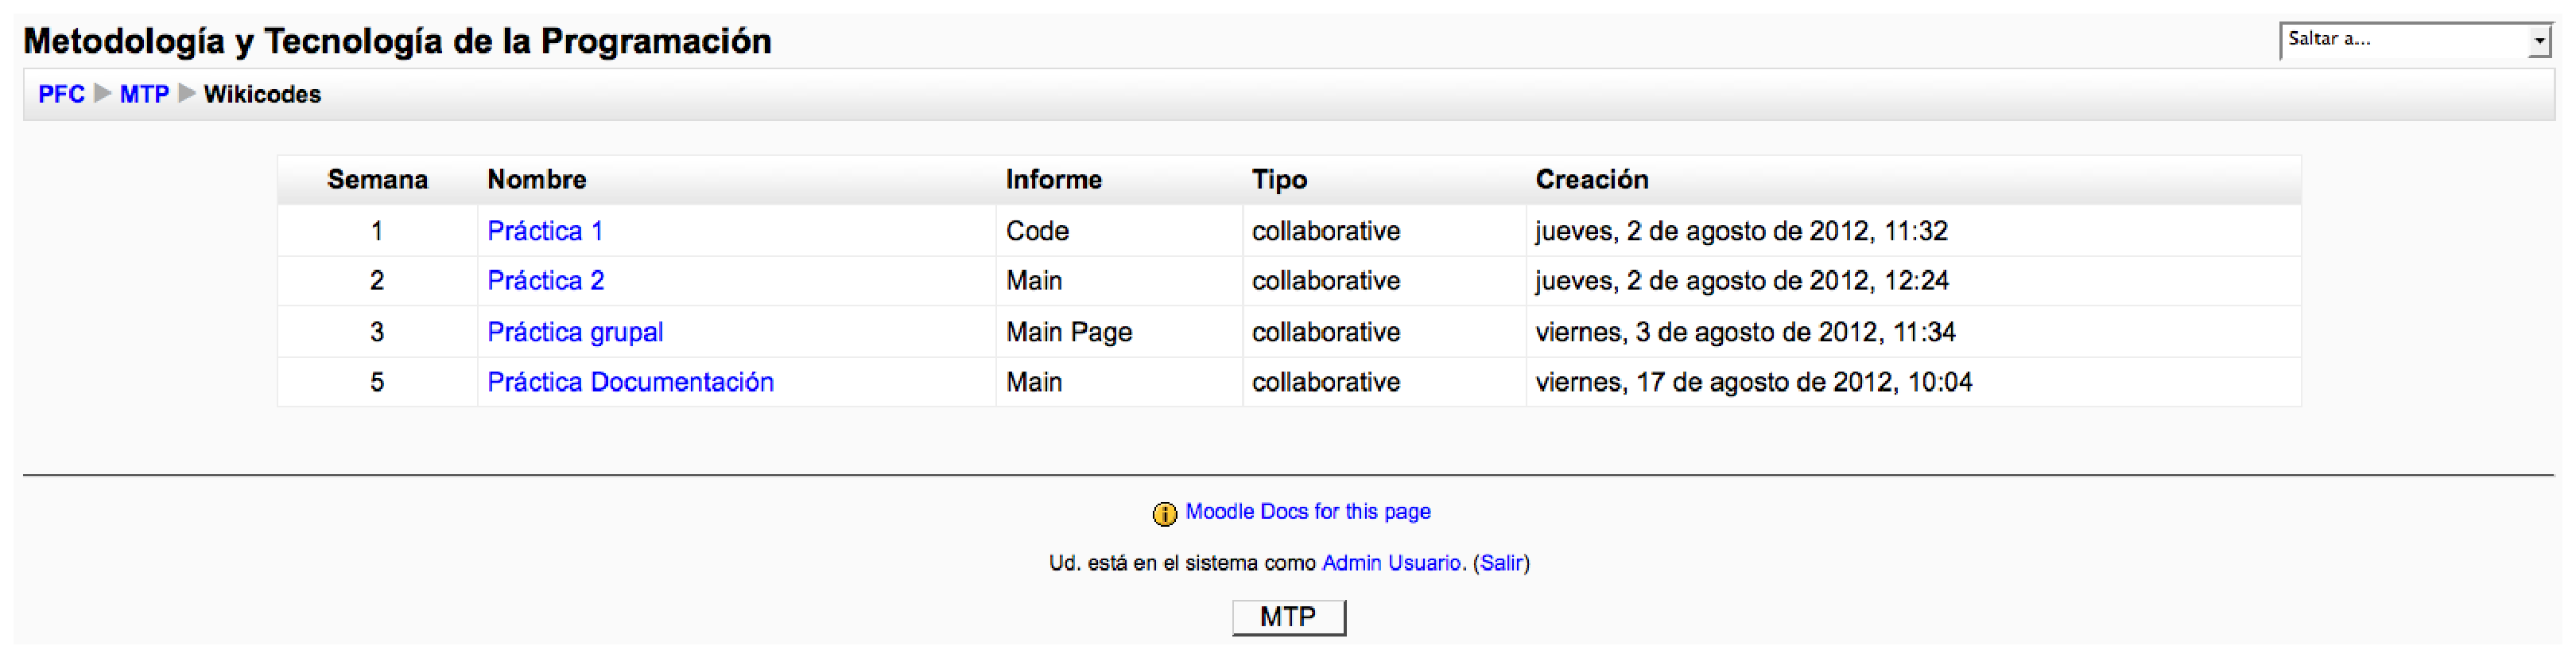
\includegraphics[width=\textwidth]{./img/v1index.eps}
	\caption{Index Wikicode v 1.x}
\end{figure}

En este listado se nos muestra información sobre todas las Wikicodes creadas.



Asimismo, tanto pulsando en la pestaña \emph{View} como accediendo desde el índice anteriormente expuesto, podemos ver el código en texto plano de cualquier Wikicode.

\begin{figure}[h]
	\label{v1view.eps}
	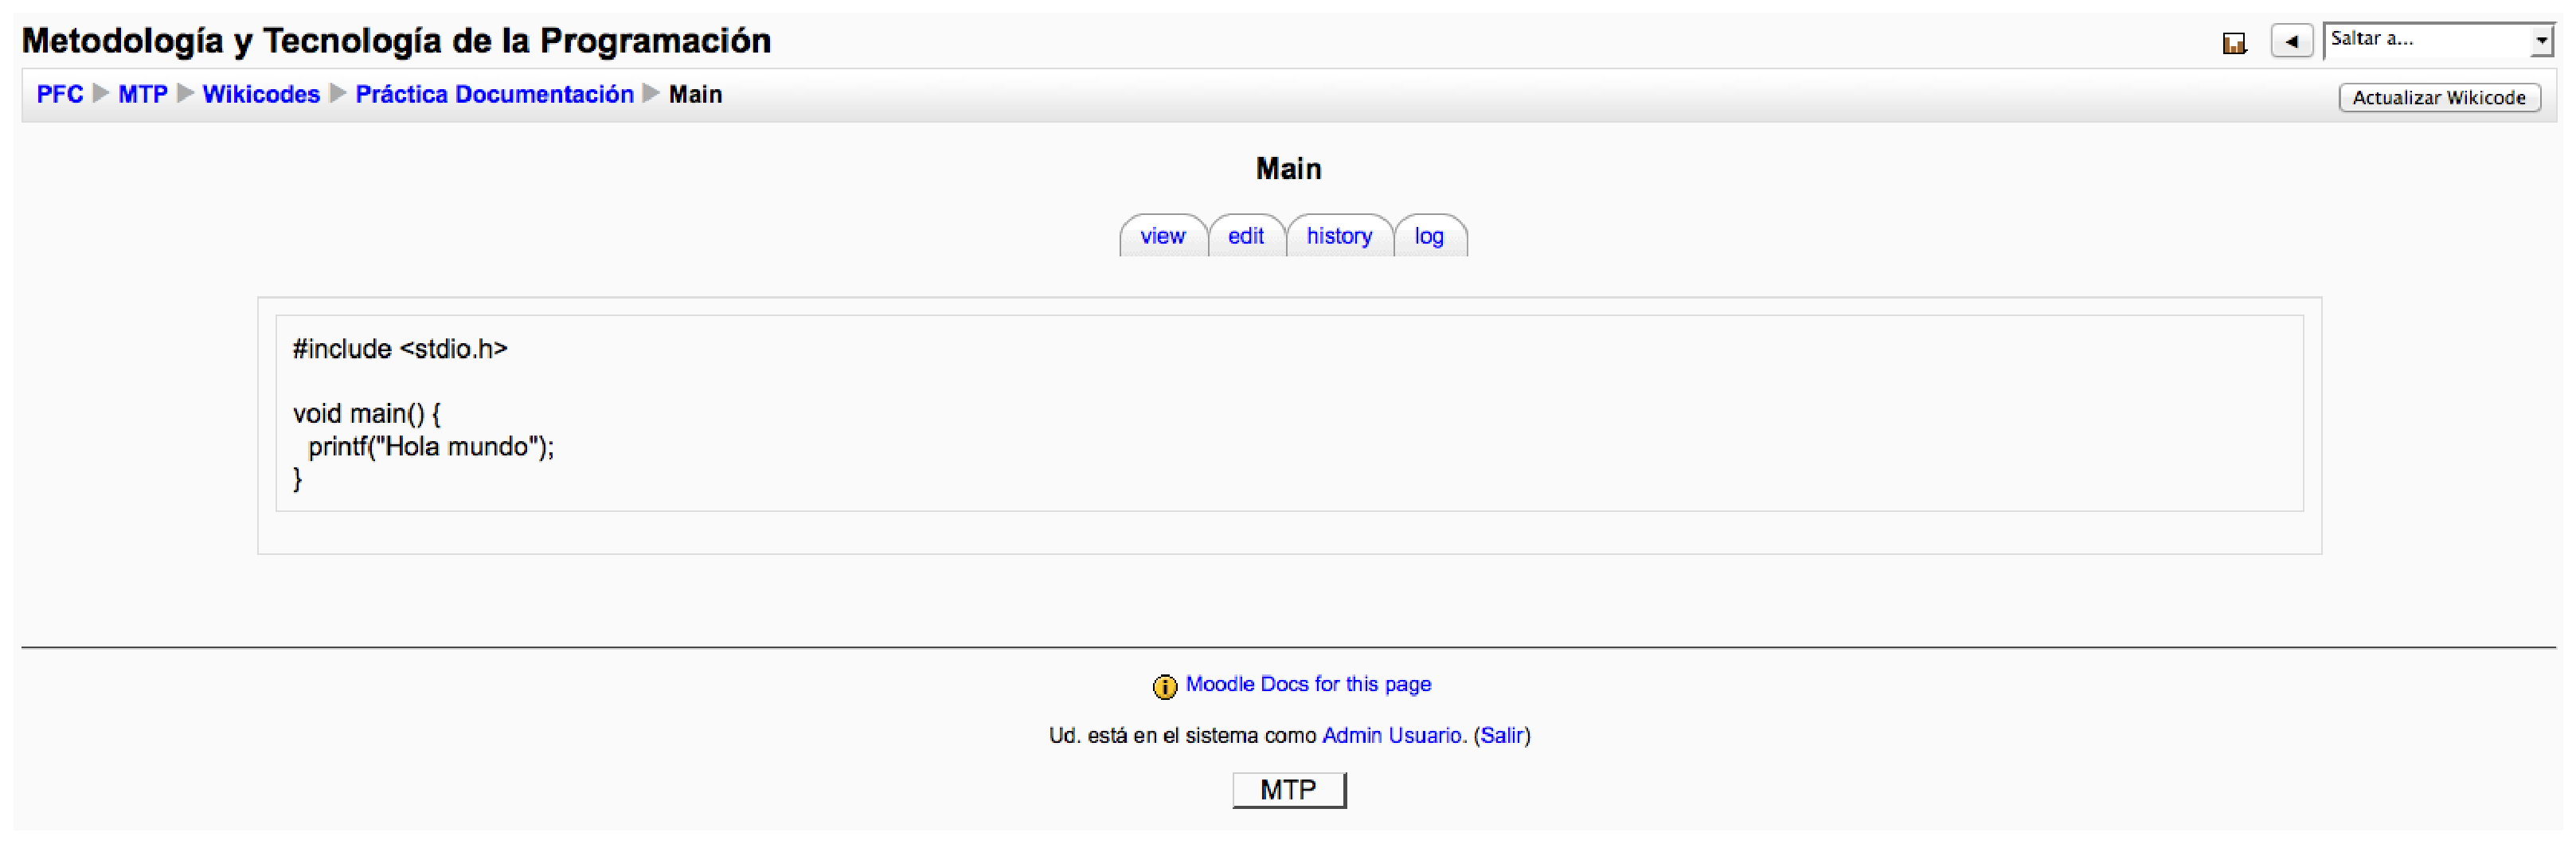
\includegraphics[width=\textwidth]{./img/v1view.eps}
	\caption{Vista en texto plano de una Wikicode v 1.x}
\end{figure}

\newpage

Por último, con respecto a esta versión, tendremos un histórico de todas las veces que hemos ido salvando nuestro código.

\begin{figure}[h]
	\label{v1history1.eps}
	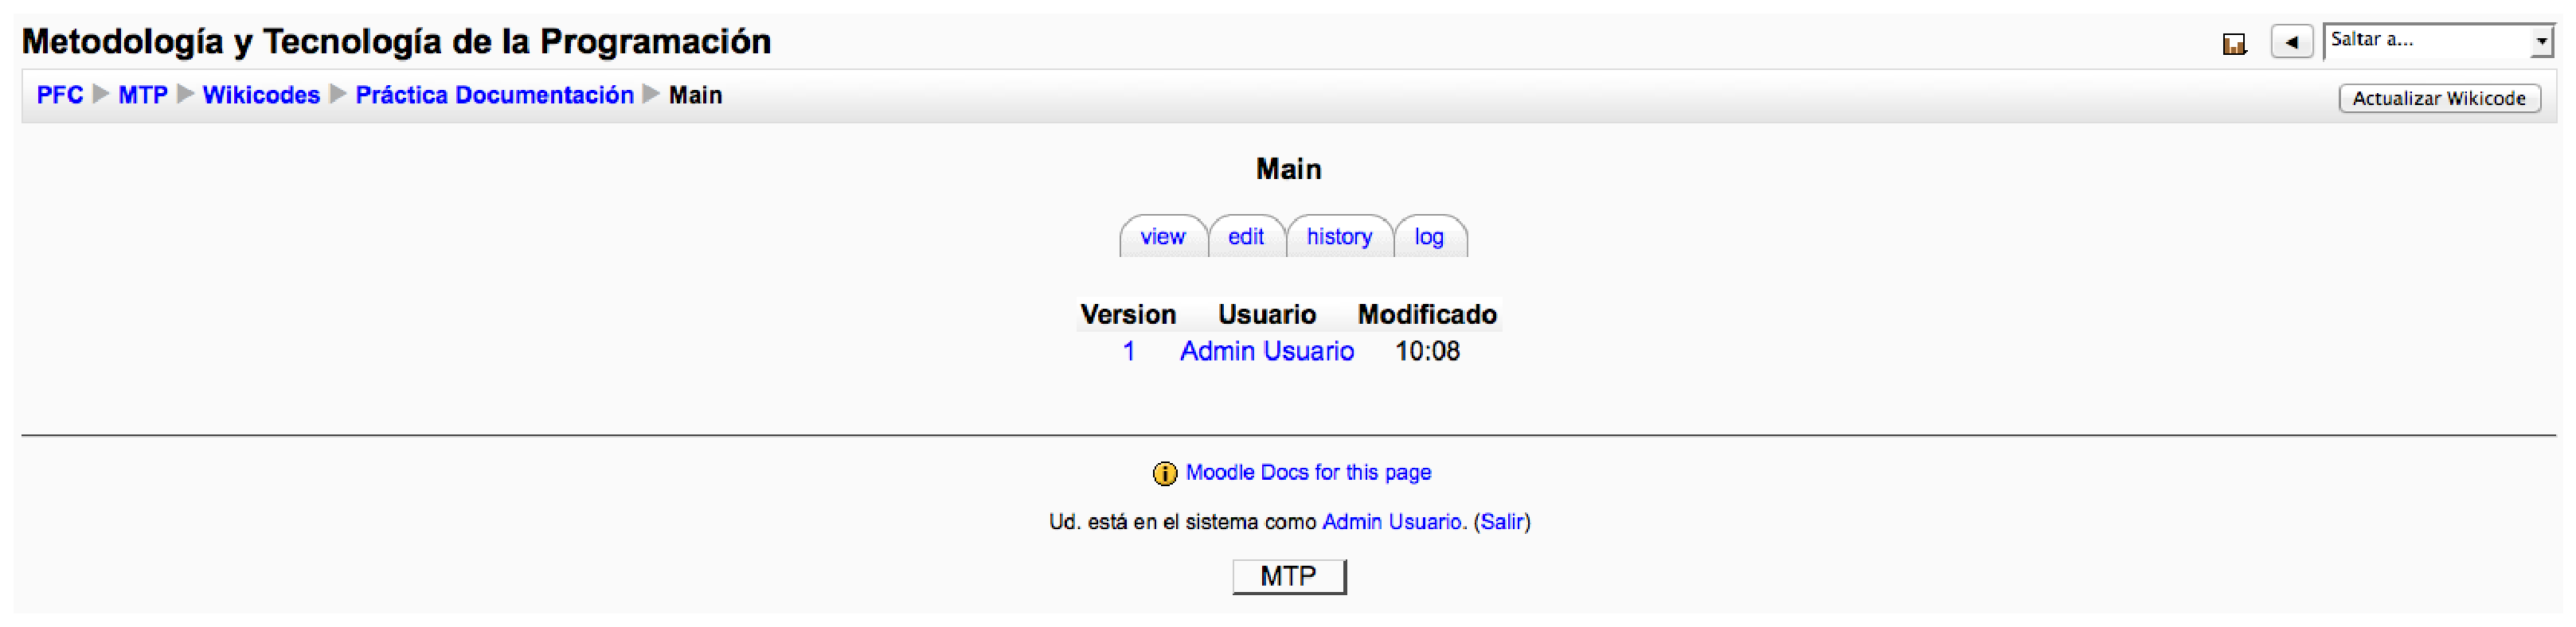
\includegraphics[width=\textwidth]{./img/v1history1.eps}
	\caption{Histórico de una Wikicode v 1.x}
\end{figure}

Si deseamos ver el contenido de una versión bastará con hacer click sobre ella y se nos mostrará una nueva ventana en la que podemos restaurar dicha versión si así lo deseamos.

\begin{figure}[h]
	\label{v1history2.eps}
	\includegraphics[width=\textwidth]{./img/v1history2.eps}
	\caption{Restaurar versión de una Wikicode v 1.x}
\end{figure}

Para restaurar una versión bastará con pulsar el enlace denominado \textbf{(Restore this version)} encuadrado en la esquina superior izquierda.

\newpage

\section{Funciones específicas de Moodle 2.x}

Para esta versión de Moodle, además de tener un interfaz más actual, gracias a la gran cantidad de nuevas librerías podemos hacer uso de funcionalidades más potentes. Estos cambios en el interfaz lo podemos ver en la pestaña \emph{View}, donde se nos muestra nuestro código fuente en formato texto plano.

\vspace{1cm}

\begin{figure}[h]
	\label{v2view.eps}
	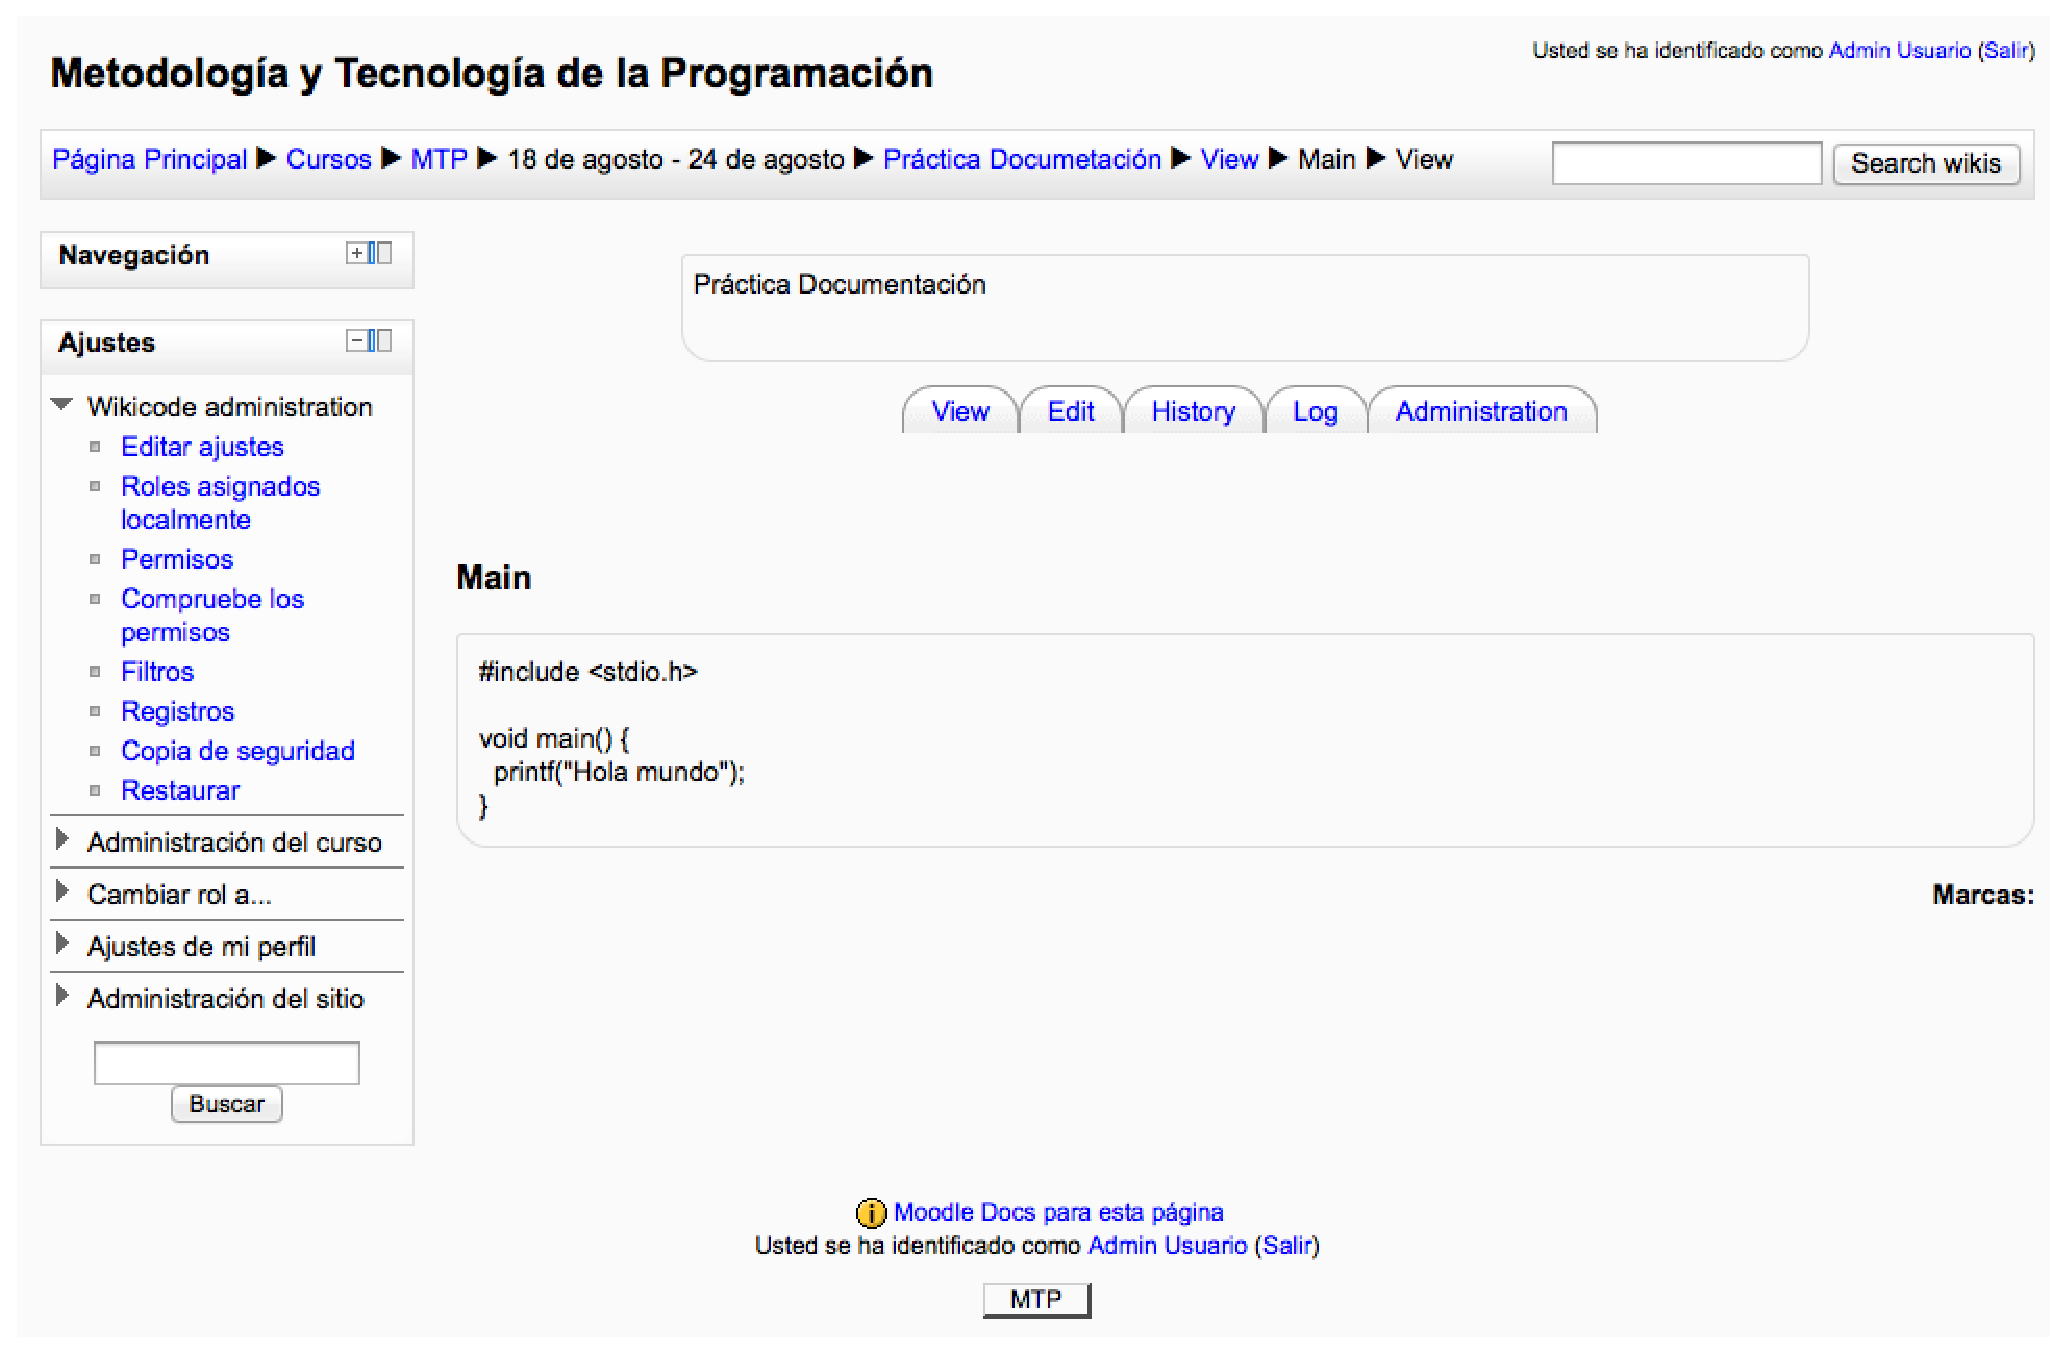
\includegraphics[width=\textwidth]{./img/v2view.eps}
	\caption{Vista en texto plano de una Wikicode v 2.x}
\end{figure}

\newpage

Sin embargo, donde más podemos notar la potencia de esta nueva versión de Moodle es en el histórico de nuestro código. Una de las ventajas principales es la posibilidad de comparar dos versiones y viendo las diferencias entre estas.

\vspace{1cm}

\begin{figure}[h]
	\label{v2history1.eps}
	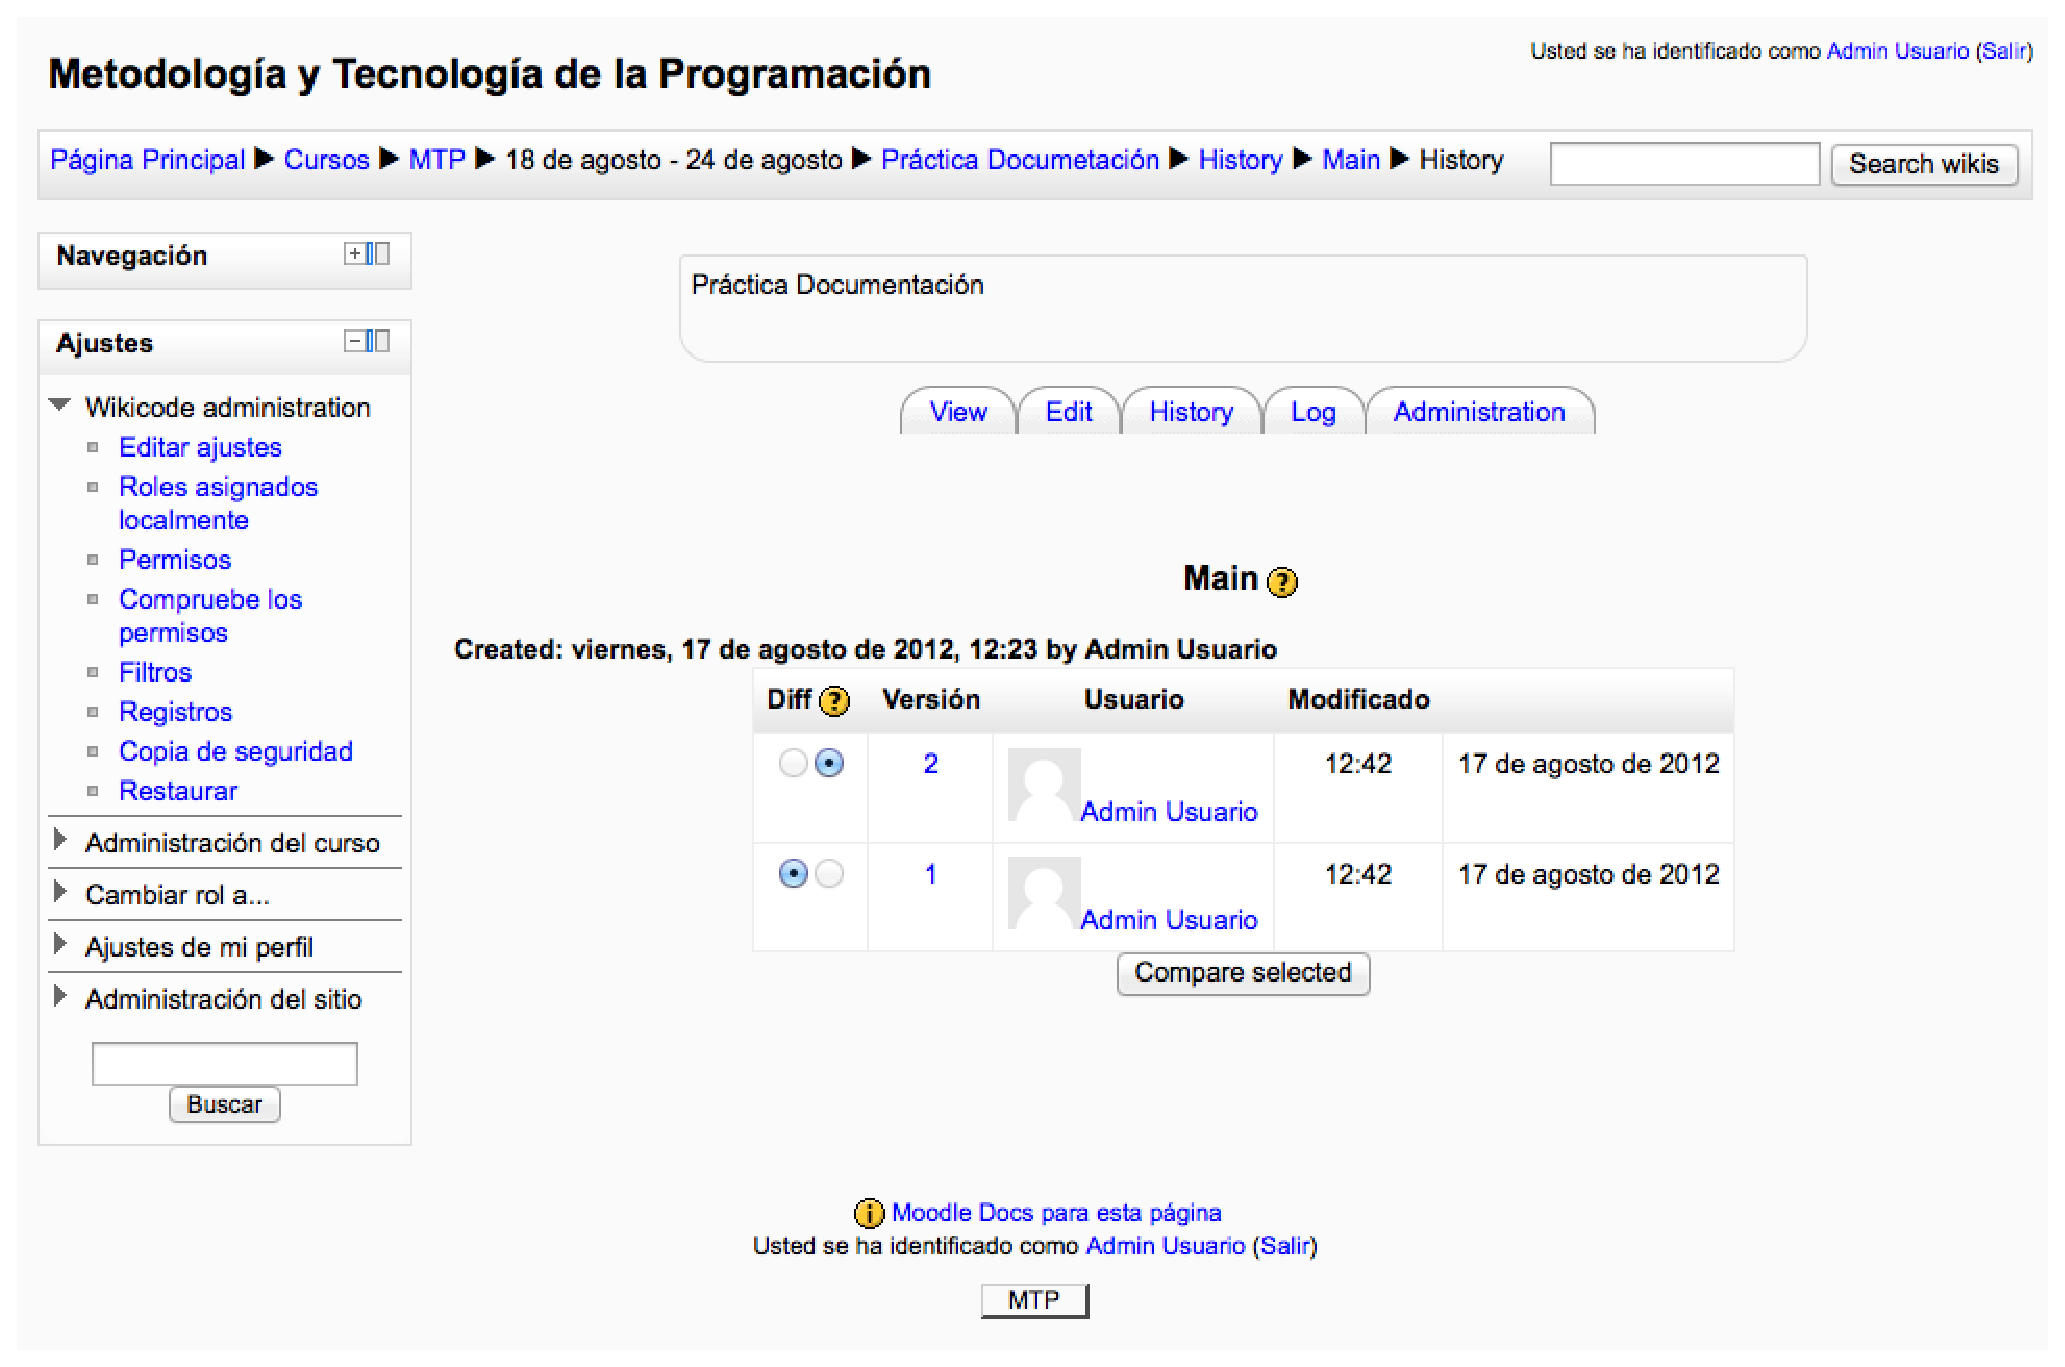
\includegraphics[width=\textwidth]{./img/v2history1.eps}
	\caption{Pantalla principal del Histórico Wikicode v 2.x}
\end{figure}

\newpage

Una vez que hayamos pulsado el botón \textbf{Compare selected}, se nos dirá la diferencia entre un código y otro.

\vspace{1cm}

\begin{figure}[h]
	\label{v2history2.eps}
	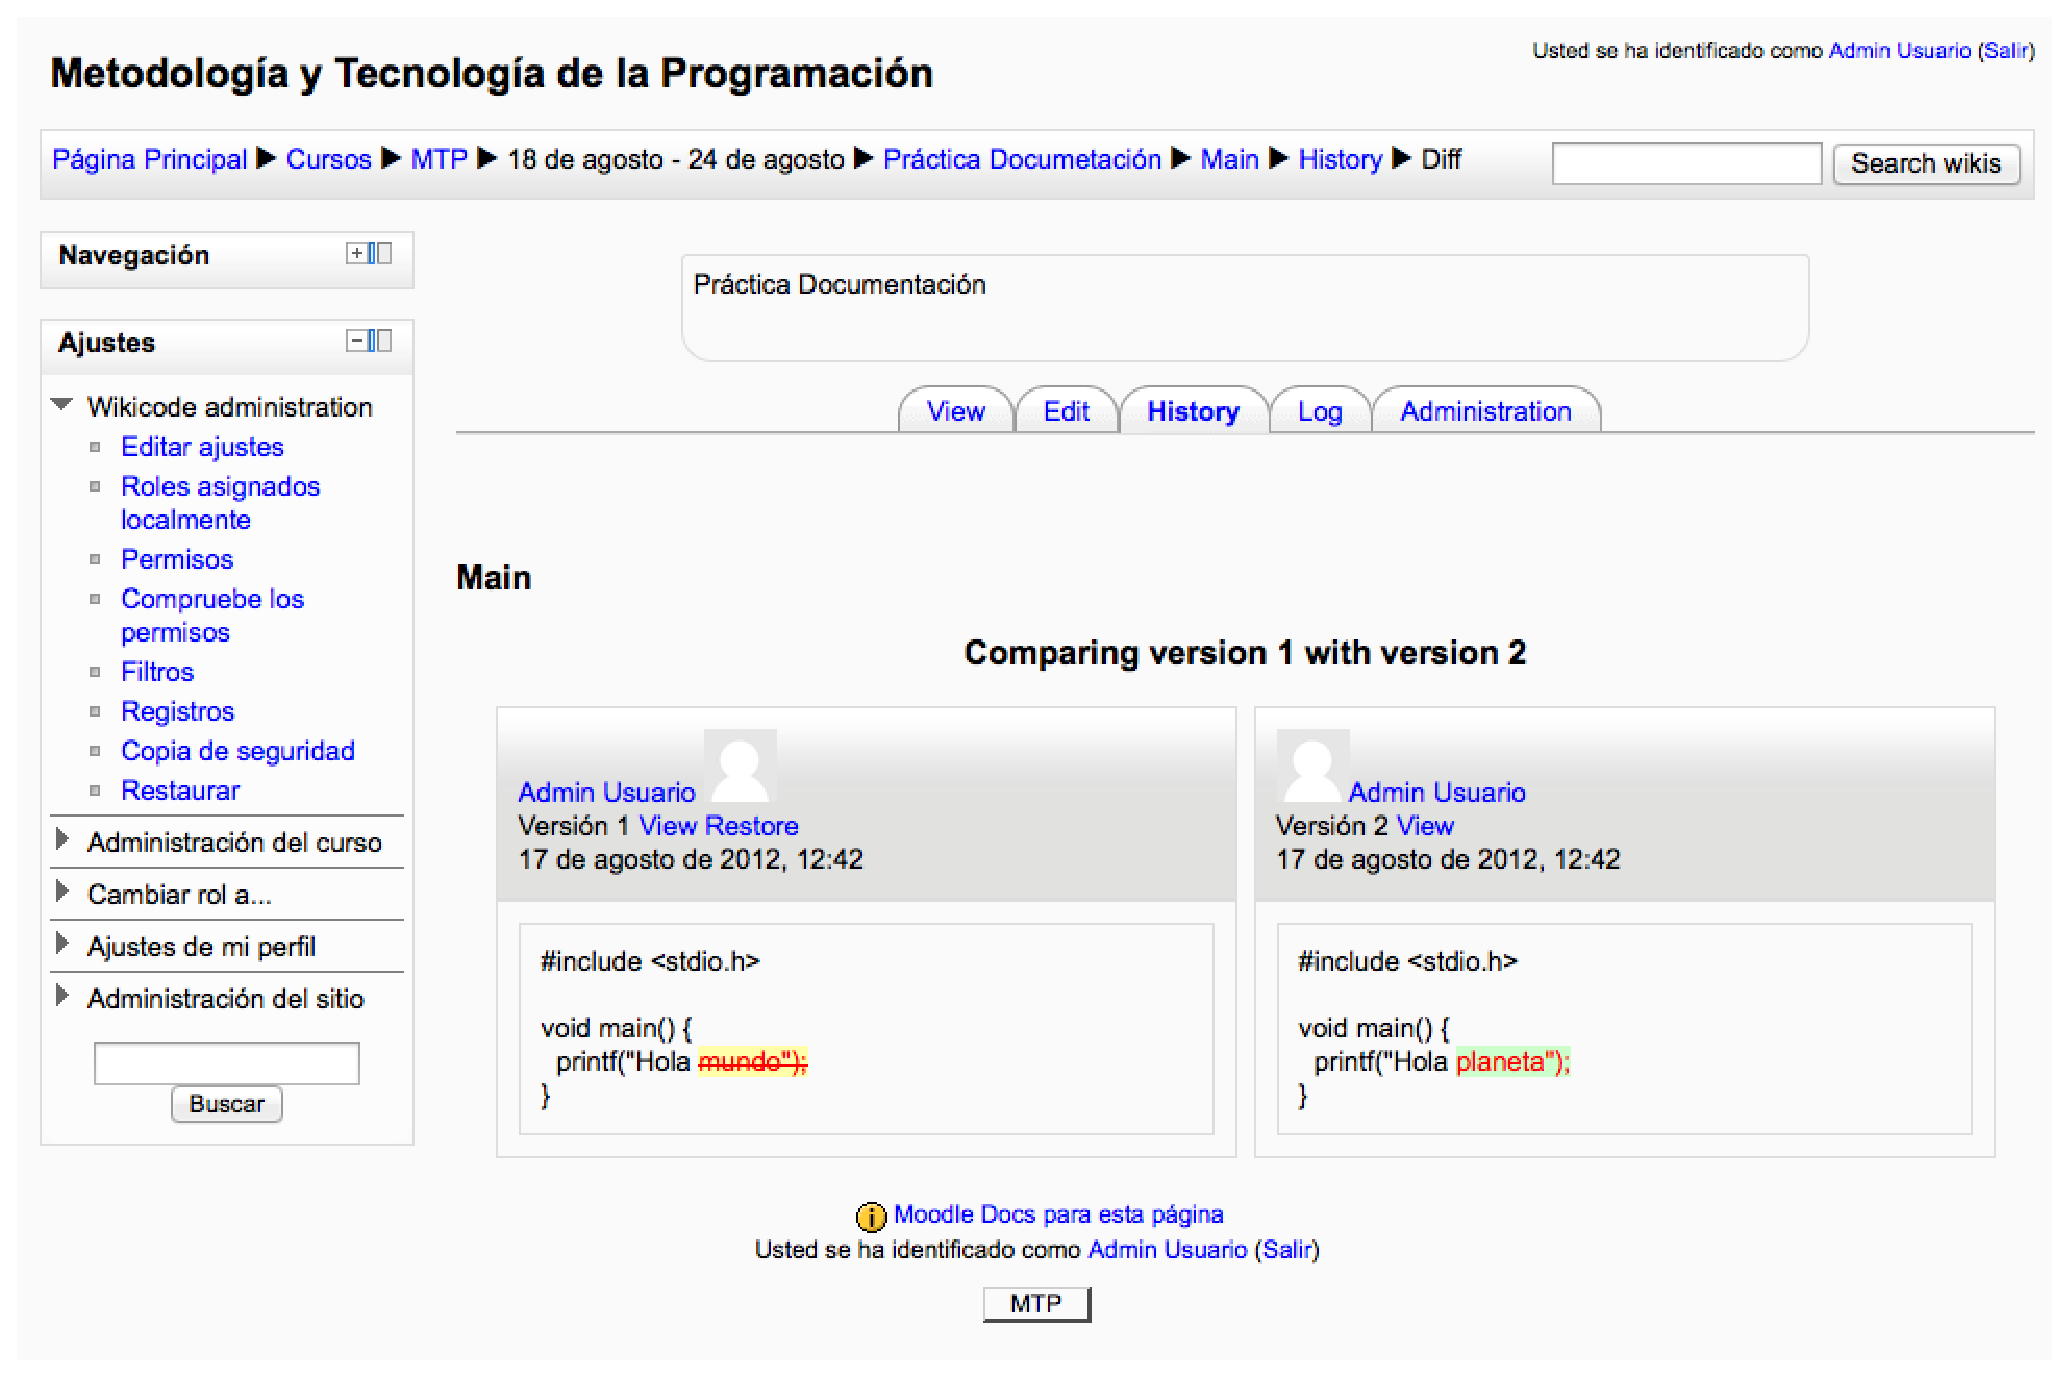
\includegraphics[width=\textwidth]{./img/v2history2.eps}
	\caption{Comparación de código. Histórico Wikicode v 2.x}
\end{figure}

\newpage

A su vez, si pulsamos sobre cualquiera de las versiones que tenemos en el histórico, además de mostrar lo que tenemos almacenado nos dará la posibilidad de restaurar dicho código pulsando el enlace \textbf{(Restore this version)}.

\vspace{1cm}

\begin{figure}[h]
	\label{v2history3.eps}
	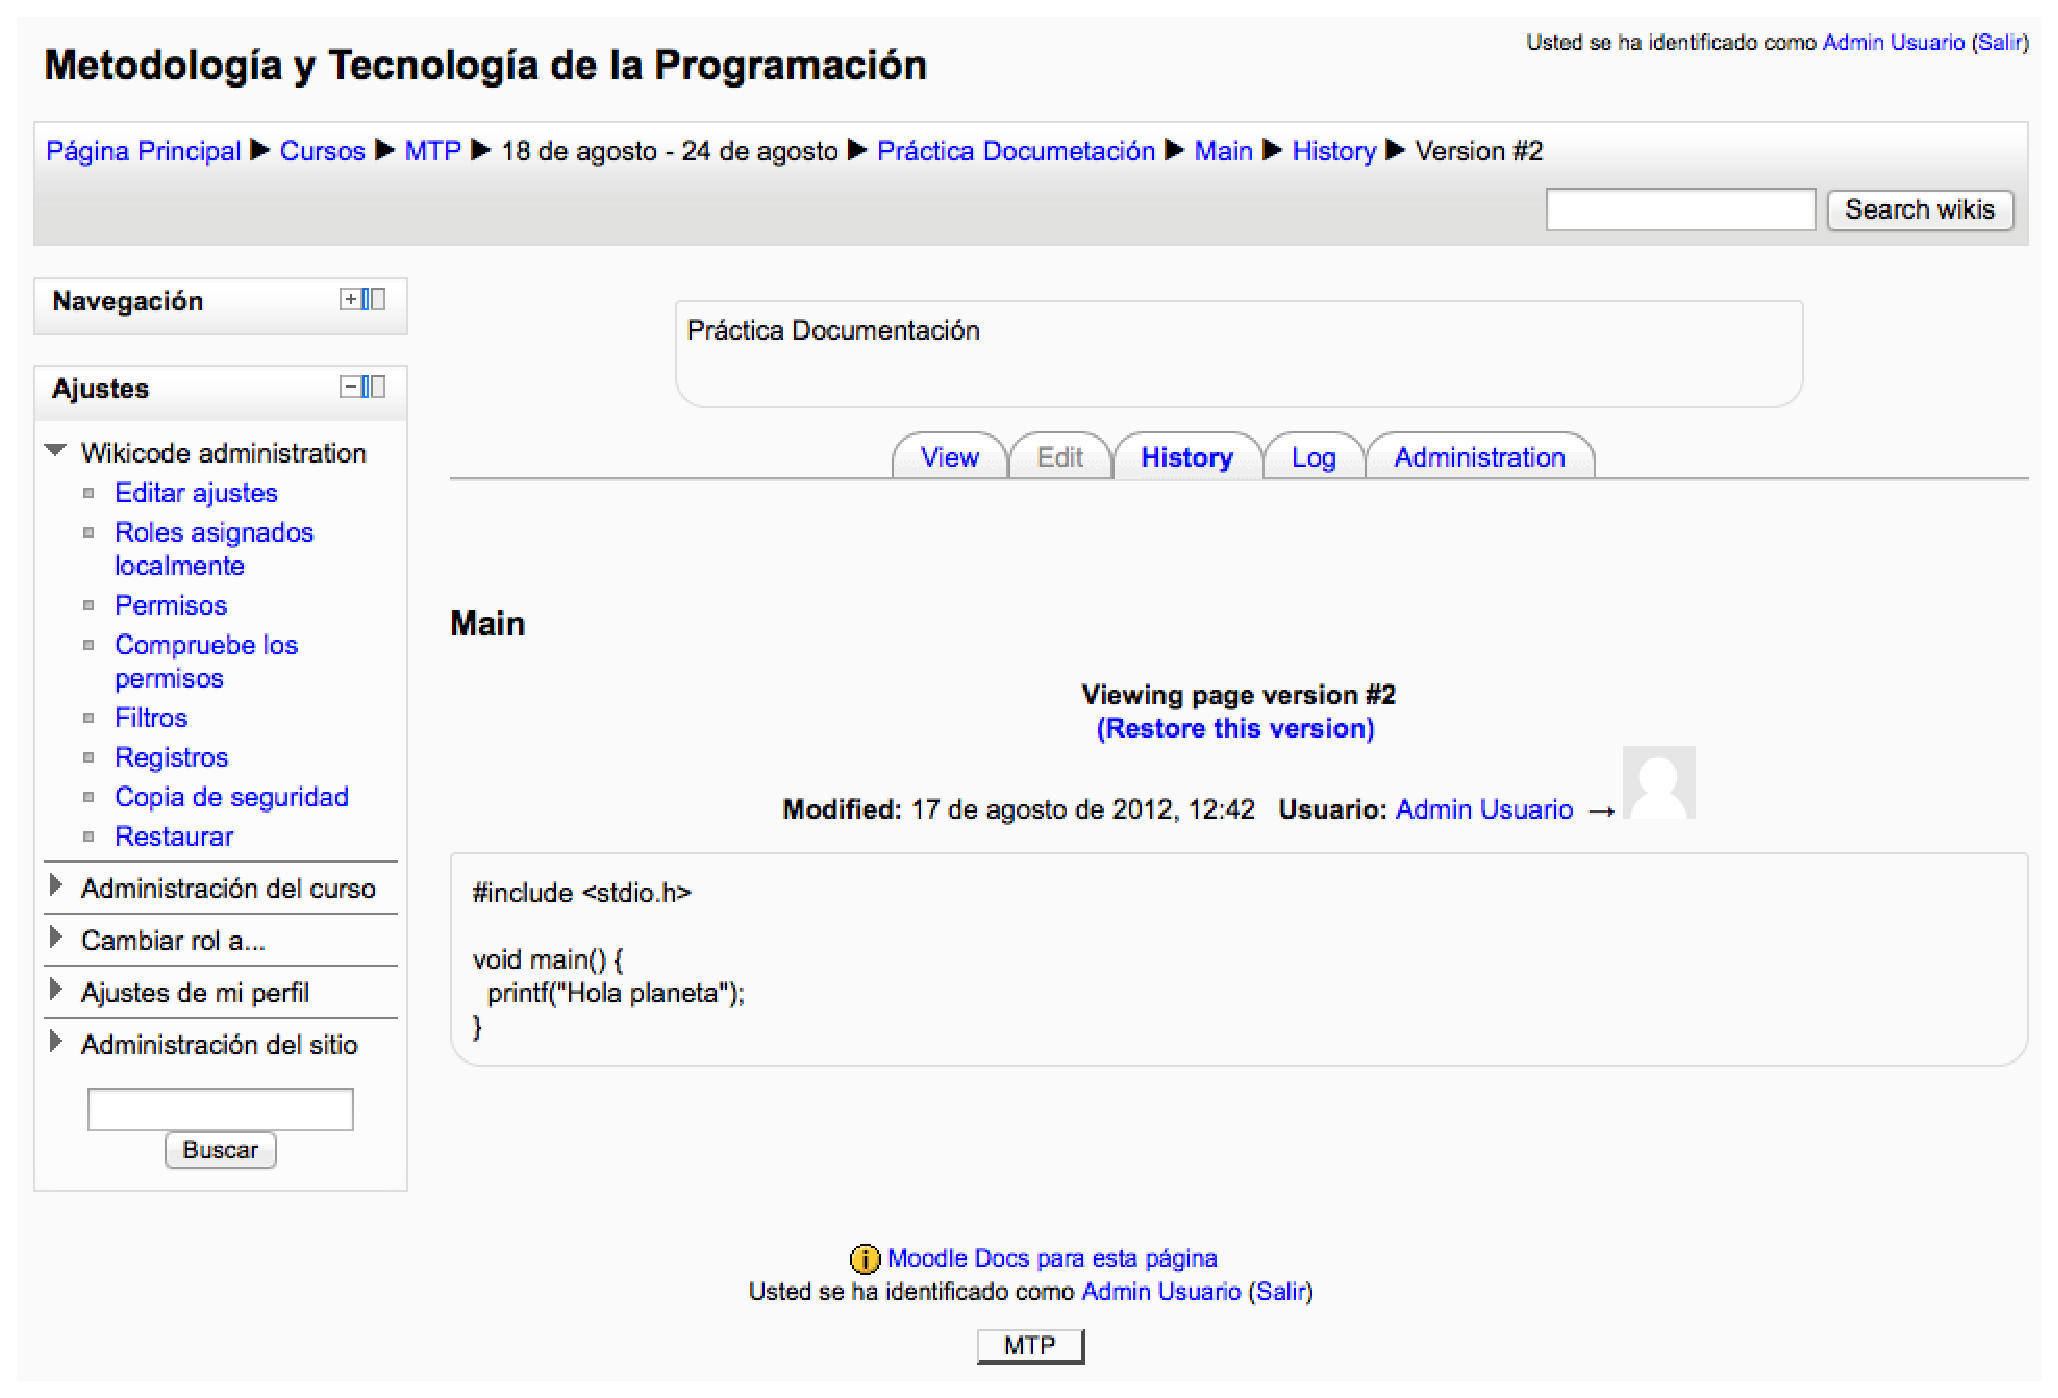
\includegraphics[width=\textwidth]{./img/v2history3.eps}
	\caption{Restaurar versión. Histórico Wikicode v 2.x}
\end{figure}

\newpage

Por último, para un usuario con el rol de administración sobre el curso, se añadirá una nueva pestaña en la que se le da la posibilidad de eliminar versiones de un histórico si así lo desea.

\vspace{1cm}

\begin{figure}[h]
	\label{v2admin.eps}
	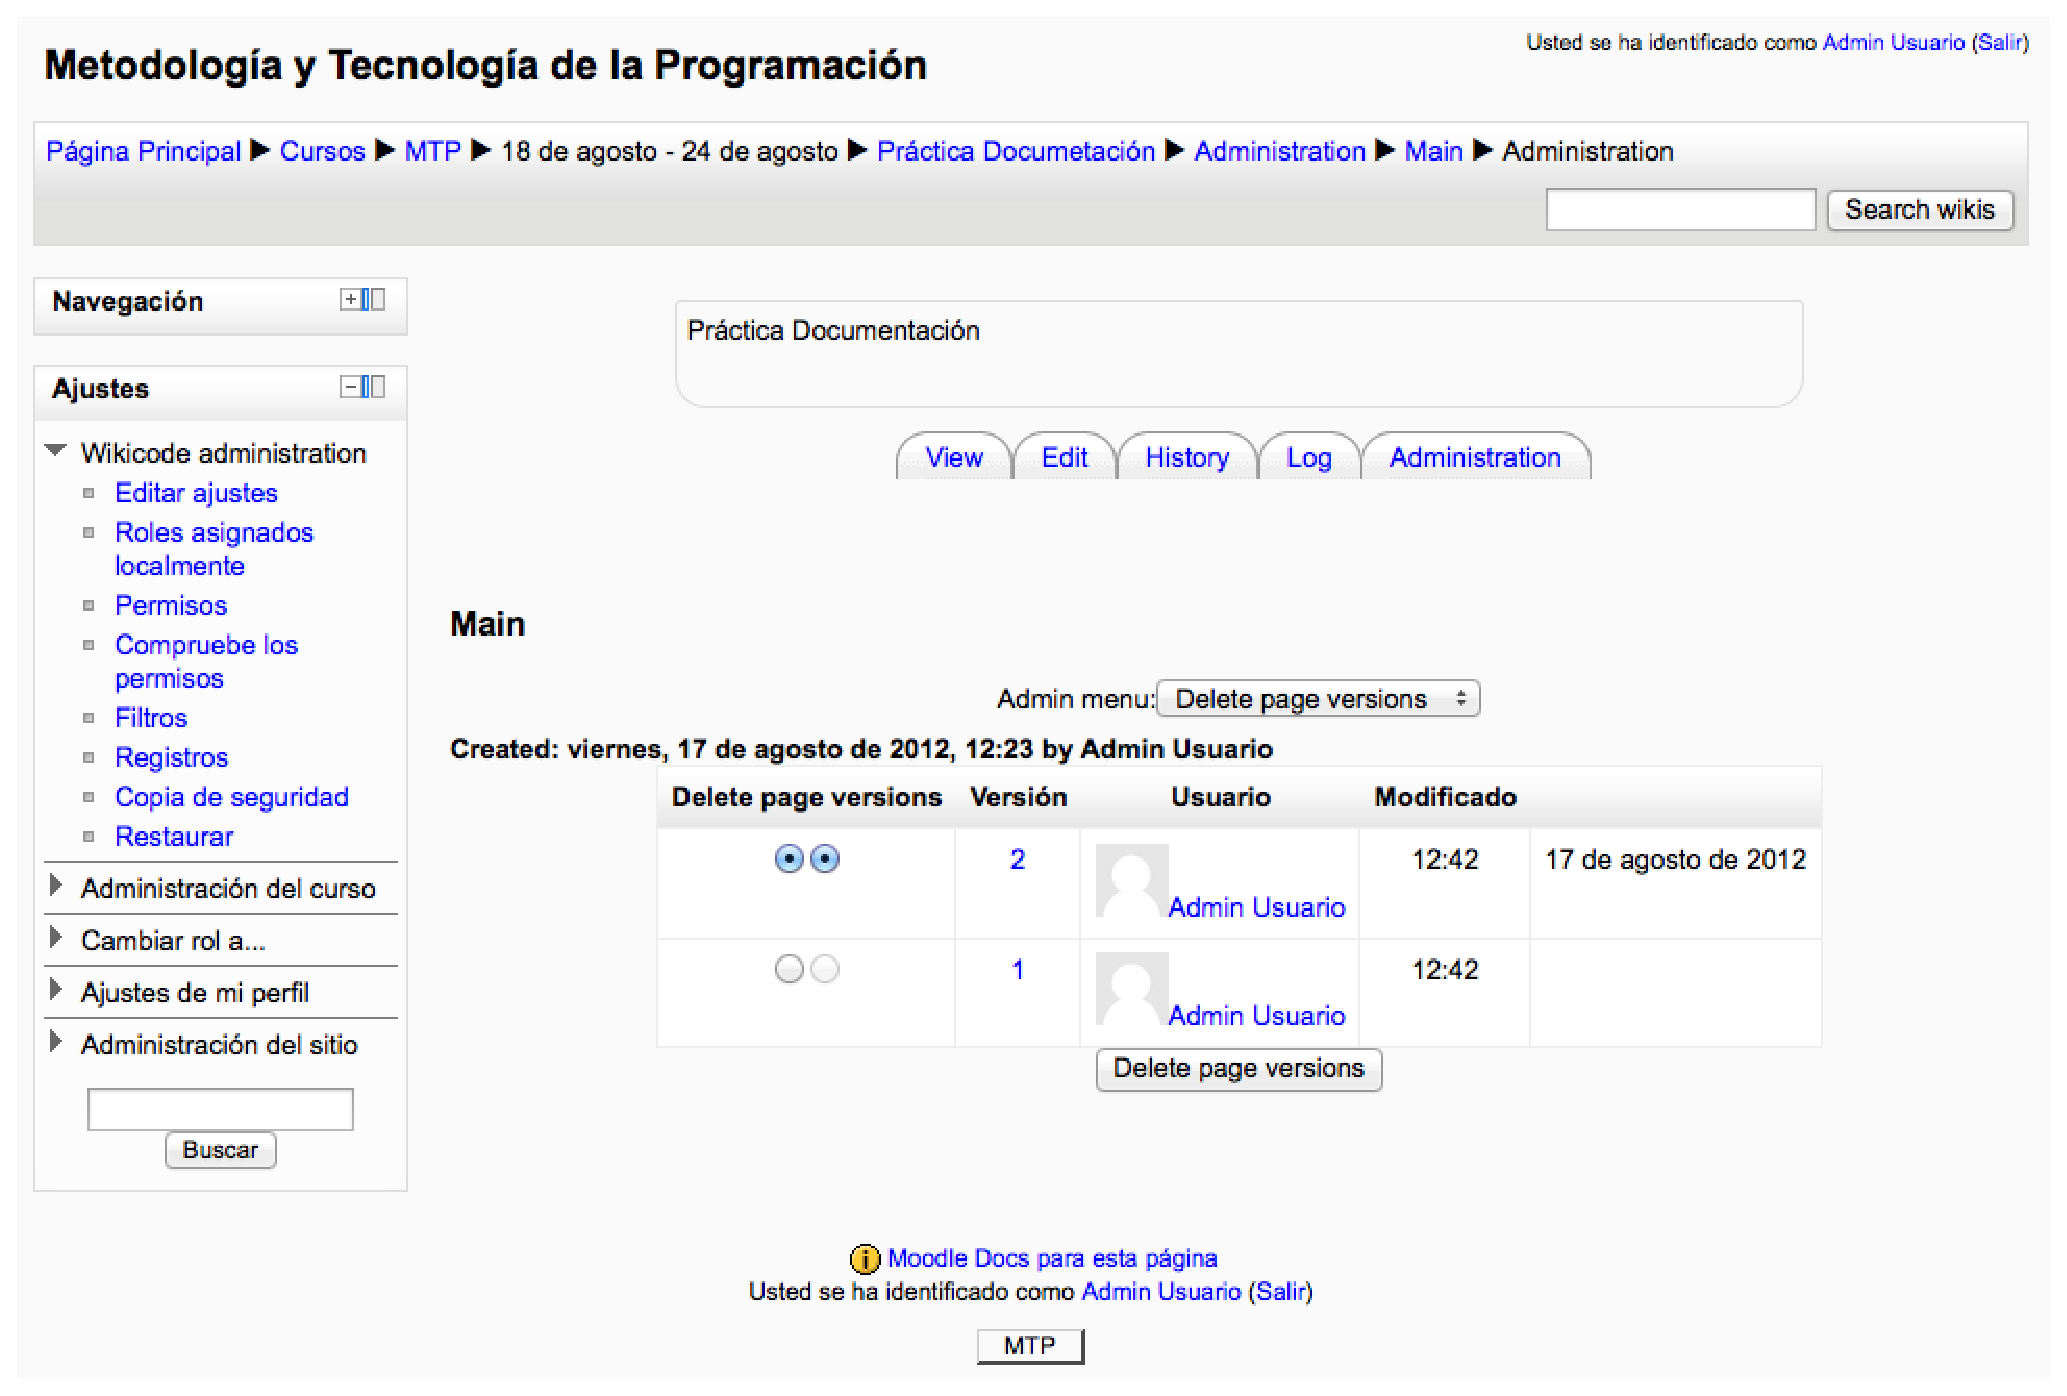
\includegraphics[width=\textwidth]{./img/v2admin.eps}
	\caption{Eliminar versión. Histórico Wikicode v 2.x}
\end{figure}

\newpage

\section{Editor}
\label{editSection}

El editor es la parte fundamental del módulo Wikicode, siendo compatible para todas las versiones de Moodle y a su vez fácilmente exportable a otros sistemas de gestión de contenidos. Se trata de un entorno de programación en lenguaje C y está dividido en tres partes las cuales se explican a continuación:

\subsection{Editor de código}

Se trata de tres botones y un editor de texto.

\begin{figure}[h]
	\label{eedit1.eps}
	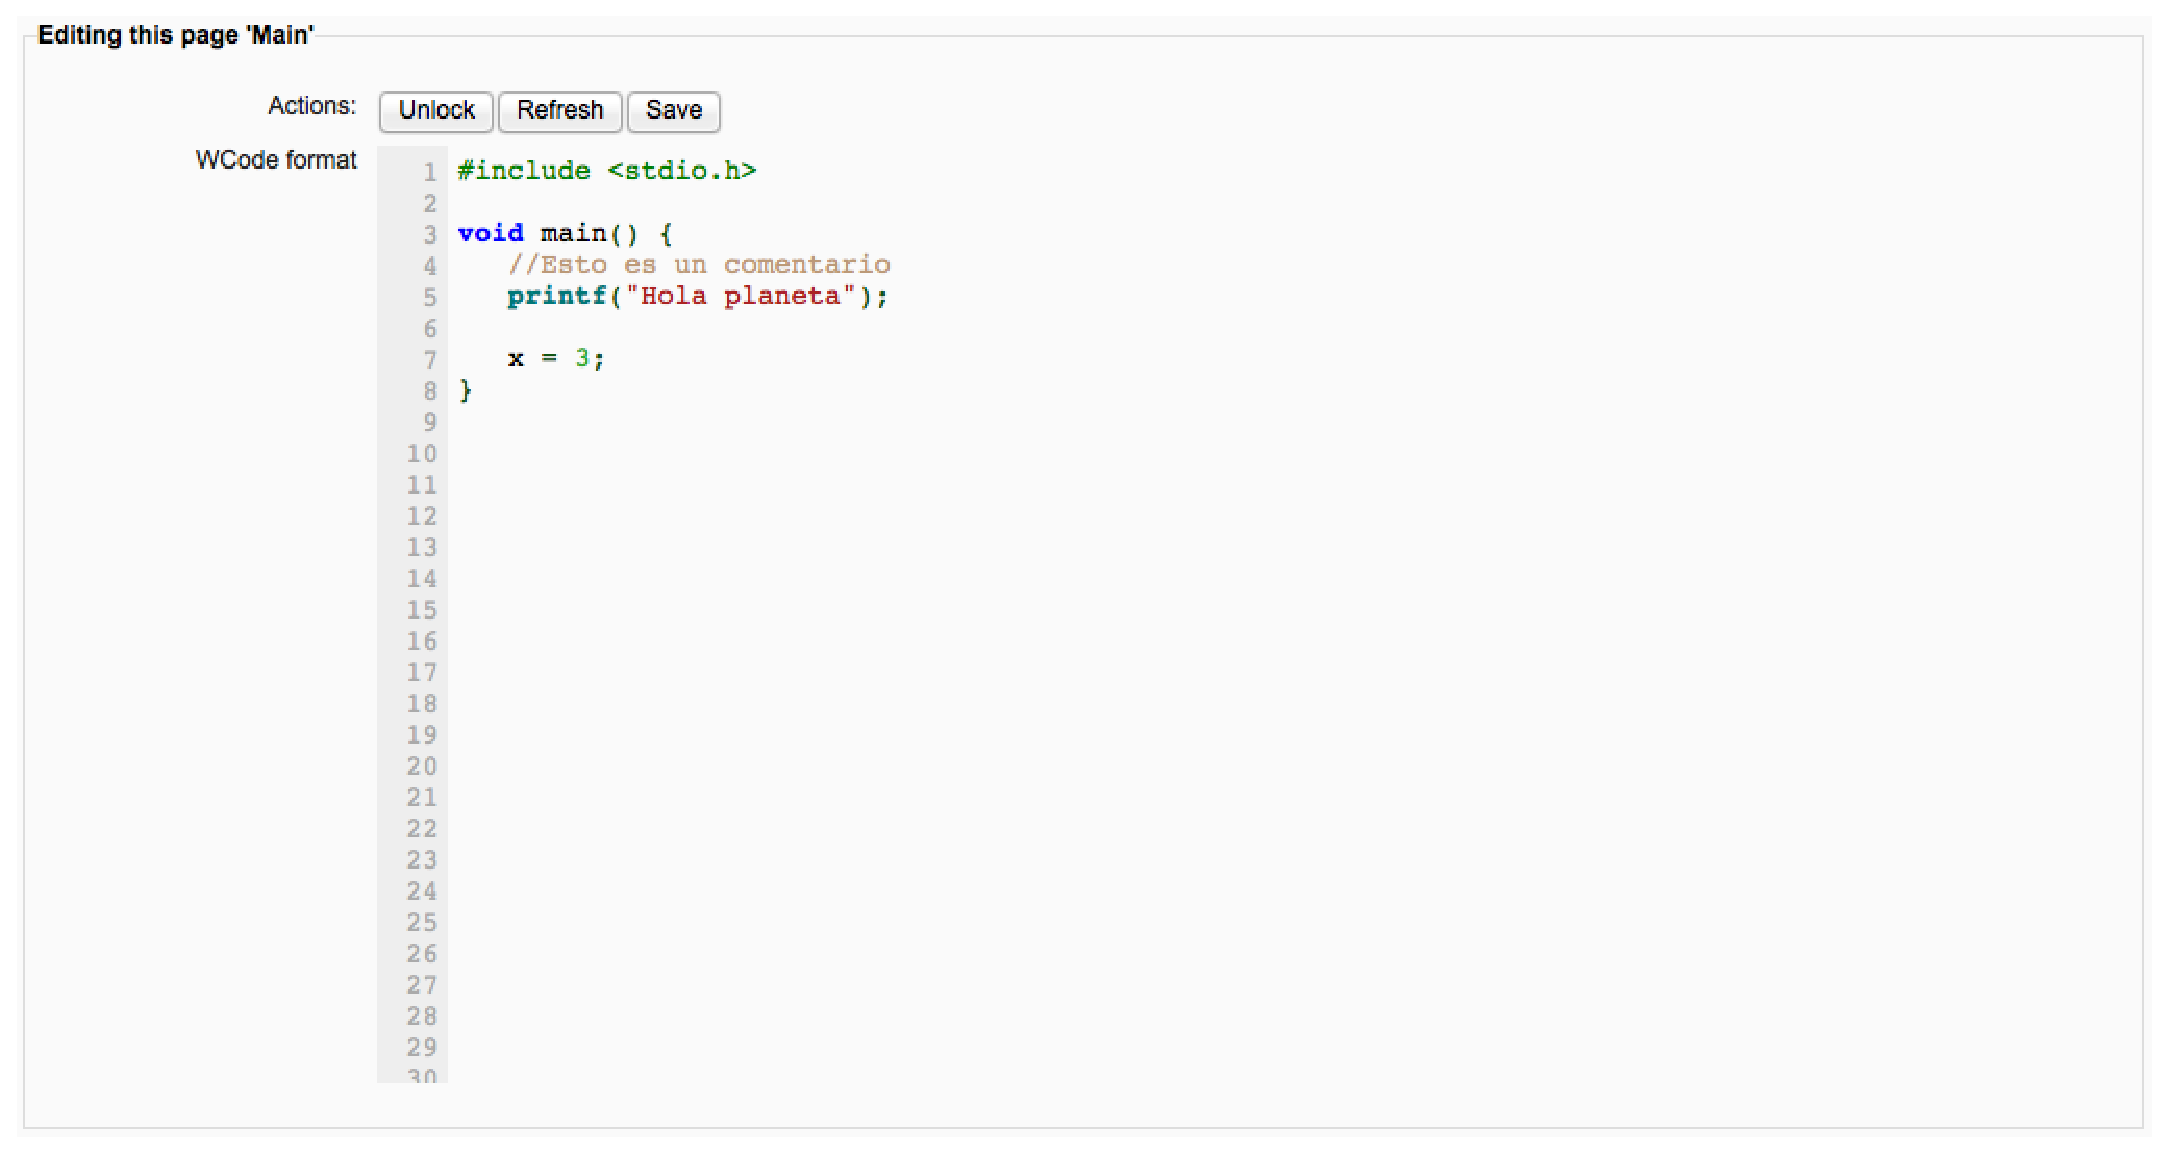
\includegraphics[width=\textwidth]{./img/eedit1.eps}
	\caption{Editor de código.}
\end{figure}

El editor es colaborativo, de modo y manera que podemos ir viendo también lo que otro usuario está programando dentro de la misma WIkicode en tiempo de ejecución. A su vez, tenemos la posibilidad de bloquear partes del código e impedir que otros usuarios la modifiquen mientras que nosotros estamos desarrollando.

El código se irá actualizando a medida que el usuario va escribiendo y el sistema va guardando la versión también de modo automático. Del mismo modo, si intentamos escribir en una parte del código bloqueada el editor nos impedirá esa acción. Las partes bloqueadas por otros usuarios están claramente diferenciadas en otro color y a su vez se nos informa que usuario es el dueño de dicha parte.

\newpage

Para comodidad del usuario final, se da formato y color al código conforme a los estándares en C siguiendo este estilo:

\begin{description}
	\item[Comentarios]: Color marrón [\#BB9977]
	\item[Palabra clave]: Color azul y tipografía en negrita.
	\item[Cadena]: Color burdeos [\#AA2222]
	\item[Números]: Color verde claro [\#3A3]
	\item[Funciones]: Color turquesa [\#077] y tipografía en negrita.
	\item[Definición]: Color verde oscuro.
	\item[Bloqueo]: Color gris claro.
\end{description}

Los botones de la parte superior de este apartado actúan del siguiente modo:

\begin{description}
	\item[Unlock]: Nos abre una ventana de estilo pop-up que nos permite desbloquear las funciones que tengamos bloqueadas del código. Podemos elegir entre una, varias o todas.

\begin{figure}[h]
	\begin{center}
	\label{eunlock.eps}
	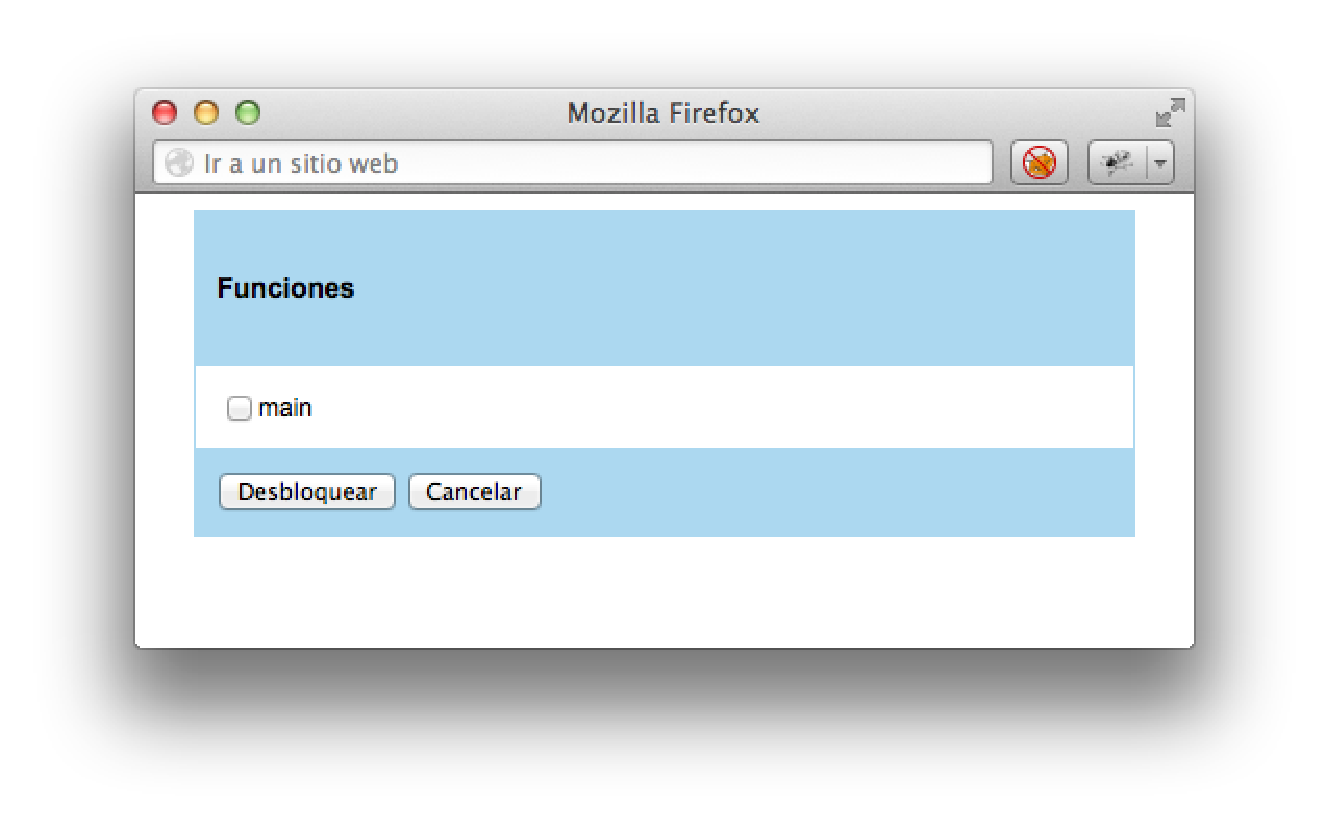
\includegraphics[scale=0.50]{./img/eunlock.eps}
	\caption{Editor de código. Pop-up de desbloqueo.}
	\end{center}
\end{figure}
	
	\item[Refresh]: Actualiza el código fuente. La actualización es semi-automática por lo que muchas veces podemos hacer esta operación manualmente.
	\item[Save]: Guarda una copia del código fuente en el histórico y desbloquea todas las funciones.
\end{description}

\newpage

Por último, el bloqueo de funciones es automático para mayor comodidad del usuario, y cada vez que modifiquemos una función el sistema internamente se encargará de bloquearla íntegramente para nosotros.

\begin{figure}[h]
	\label{fig:eedit2}
	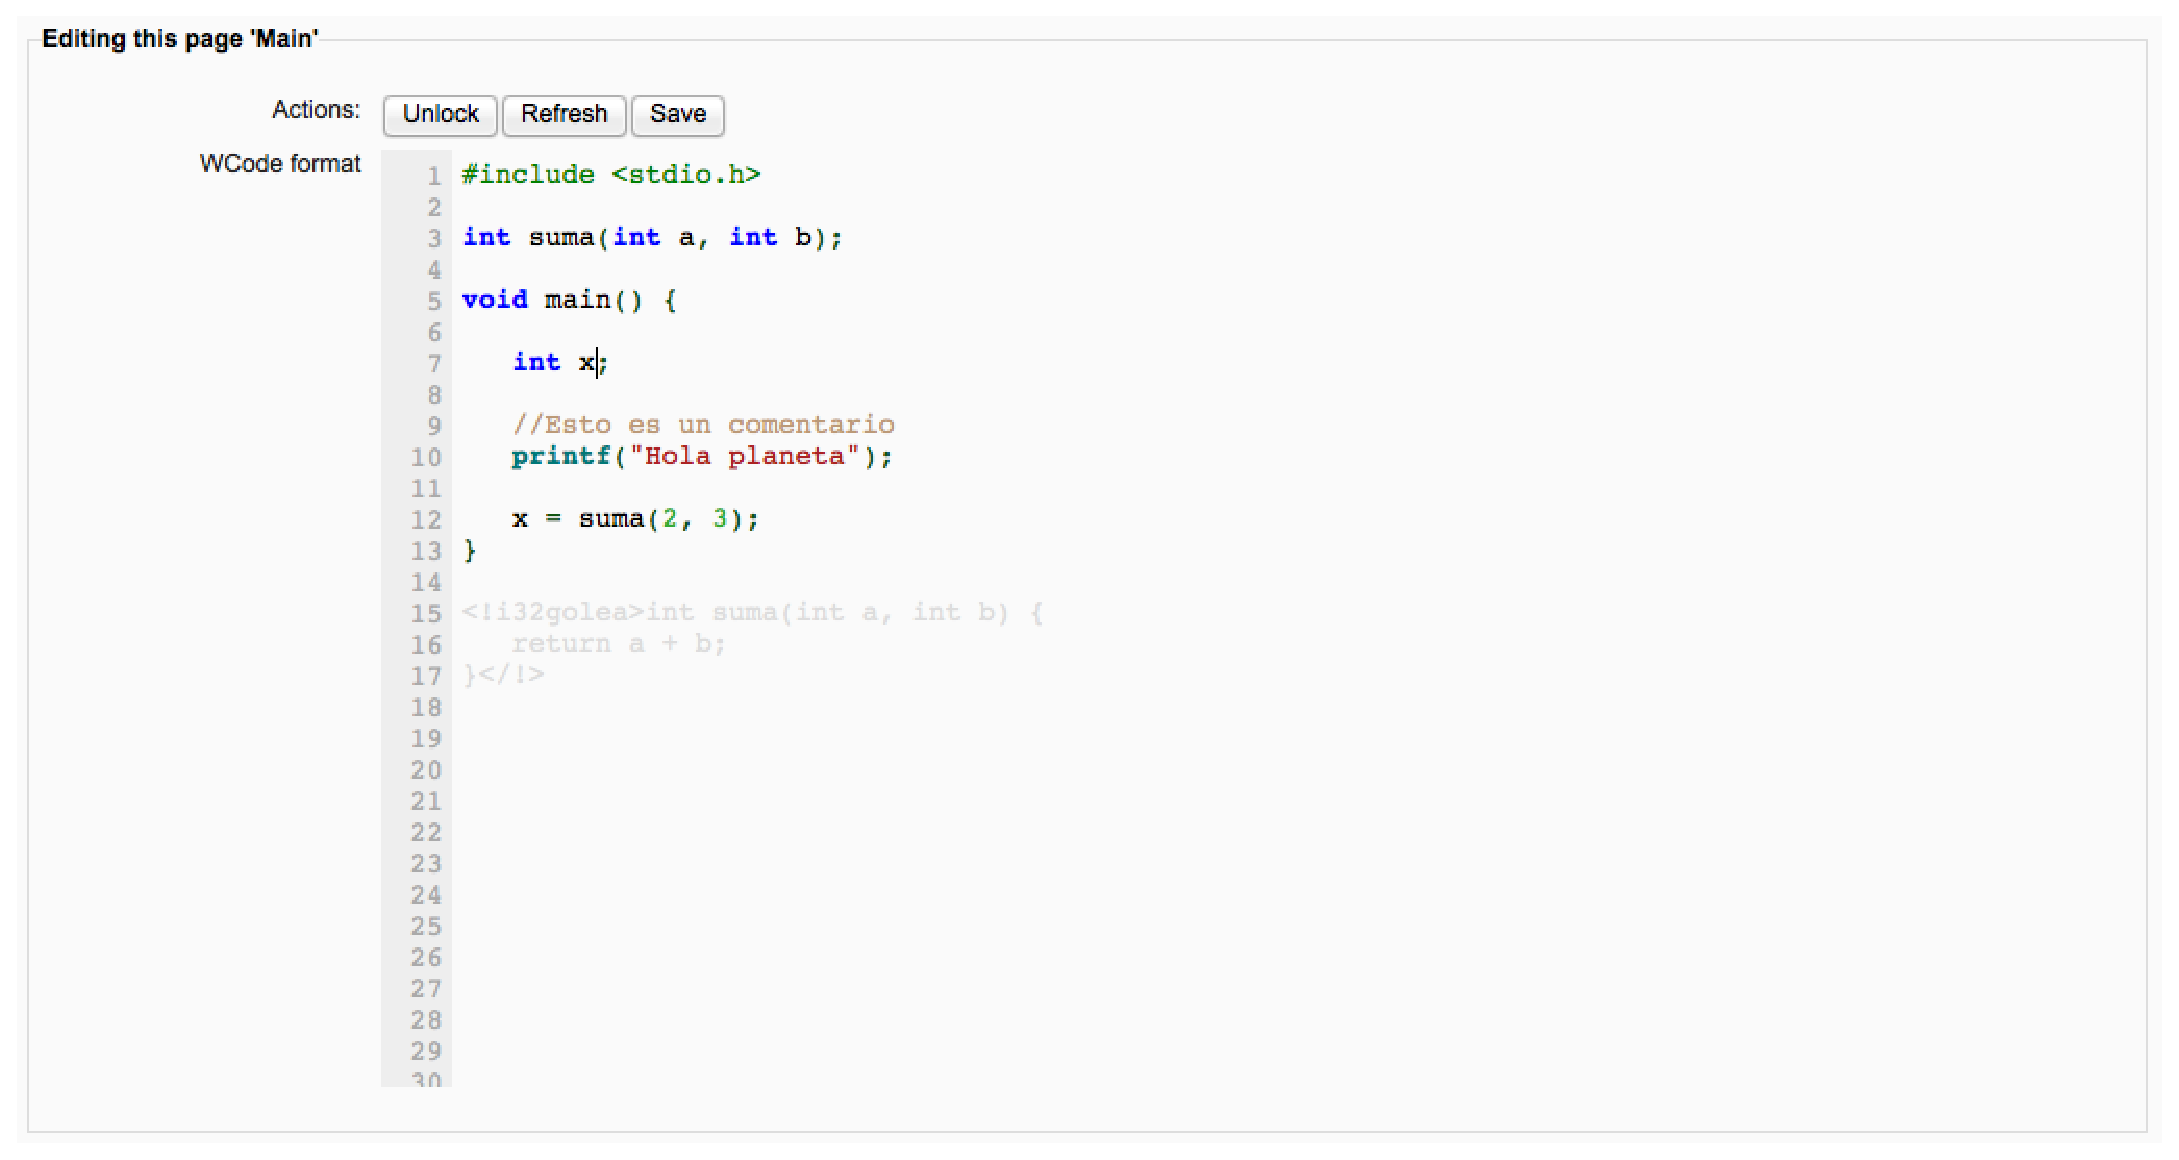
\includegraphics[width=\textwidth]{./img/eedit2.eps}
	\caption{Editor de código. Bloqueo por otro usuario.}
\end{figure}

Como podemos ver en la figura 3.20, el usuario \textbf{i32golea} ha bloqueado la función \emph{suma}. Hasta que dicho usuario no la desbloquee no se nos permitirá modificar dicha función, sin embargo podemos ir viéndola y compilando ésta a medida que el usuario vaya modificándola. 

\newpage

\subsection{Chat}

Para facilitar la interacción entre los usuarios que estén modificando una \emph{Wikicode}, se ha dotado a esta pestaña de Edición de un apartado para que puedan comunicarse entre ellos. Dicha comunicación de manera escrita será instantánea, se mantendrá el histórico por si algún usuario no está presente en ese momento y podemos ver claramente cuando y quien se comunicó con el grupo.

\begin{figure}[h]
	\label{fig:echat}
	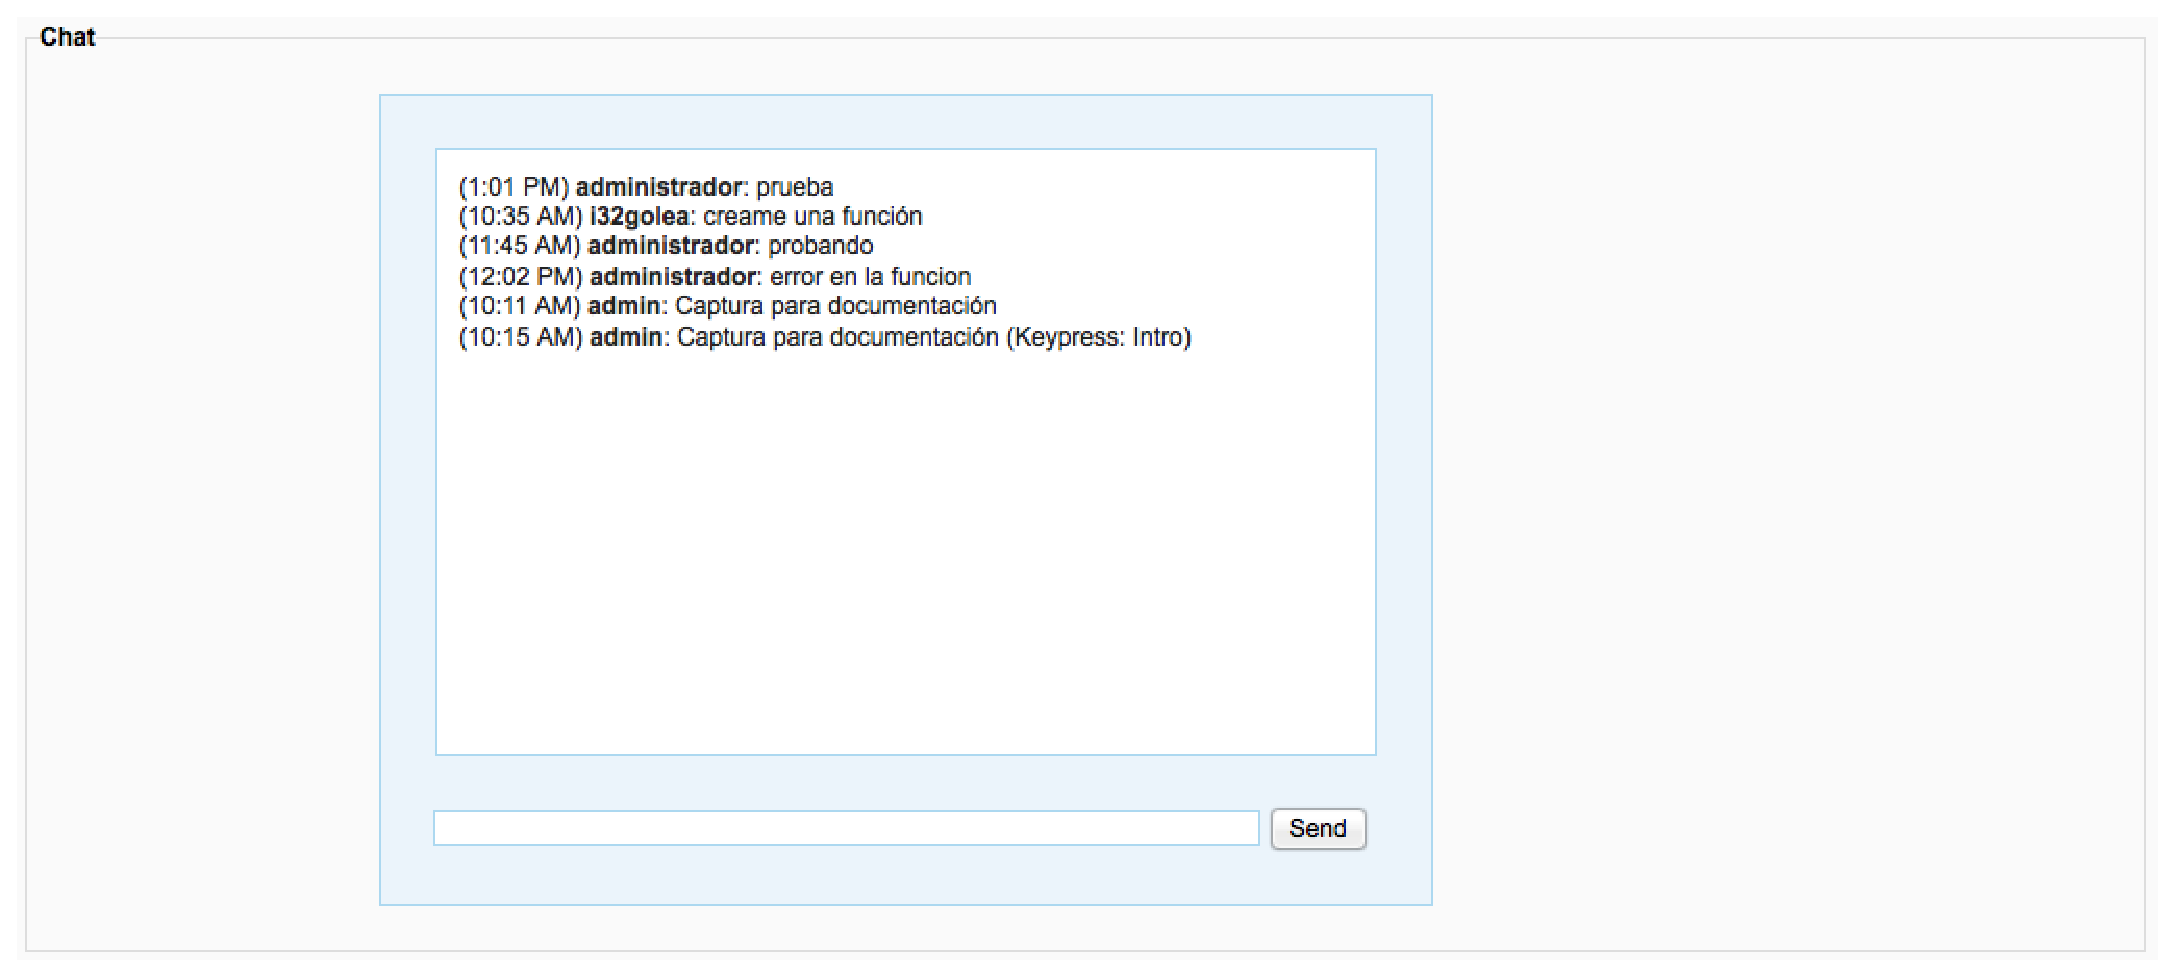
\includegraphics[width=\textwidth]{./img/echat.eps}
	\caption{Editor de código. Chat.}
\end{figure}

\newpage

\subsection{Compilador}

Por último, en la subsección que se refiere a la compilación del código se pueden distinguir dos partes. En la superior se nos mostrarán una serie de mensajes y en la inferior tenemos una serie de botones cuya funcionalidad es la siguiente:

\begin{description}
	\item[Compile]: Llamamos al compilador que hemos configurado a la hora de crear la \emph{Wikicode} (Figura 3.5) pasándolo como argumento el código fuente. Si hay errores de compilación se nos mostrarán en el cuadro de texto superior al botón y el contador de errores en el log aumentará en uno (Figura 3.8). Si no hay errores se nos mostrará un mensaje informándonos de ello.
	
	\begin{figure}[h]
		\label{fig:ecompile1}
		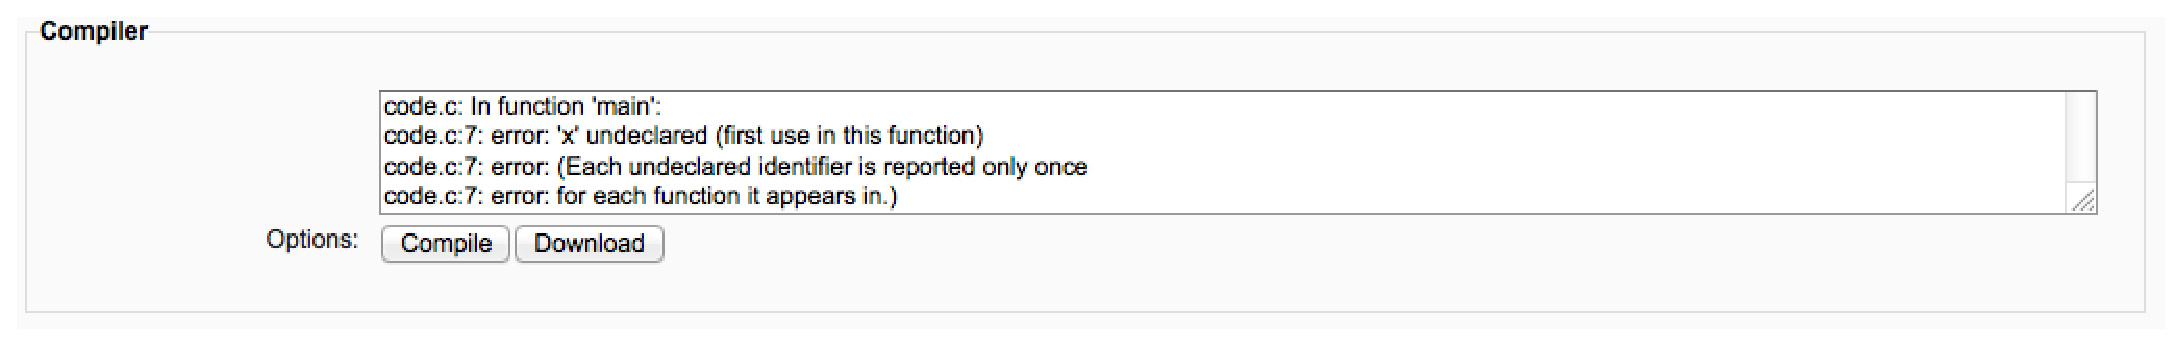
\includegraphics[width=\textwidth]{./img/ecompile1.eps}
		\caption{Editor de código. Error de compilación.}
	\end{figure}
	
	\item[Download]: Si la compilación es correcta se nos da la posibilidad de descargar el ejecutable creada. Si nuestro OS es \emph{Windows} se descargará el ejecutable compilado con el configurado en la opción \emph{Windows Compiler Path} (Figura 3.5). Si nuestro OS está basado en UNIX se descargará el ejecutable compilado con el marcado en la opción \emph{Unix Compiler Path} (Figura 3.5). Esto nos permite usar \emph{Cross Compiler}\footnote{\textbf{Cross Compiler:} Compilador capaz de crear ejecutables para una plataforma diferente a la que está ejecutándose.} independientemente del OS que esté instalado el servidor.
\end{description}

\begin{figure}[h]
	\begin{center}
	\label{fig:ecompile}
	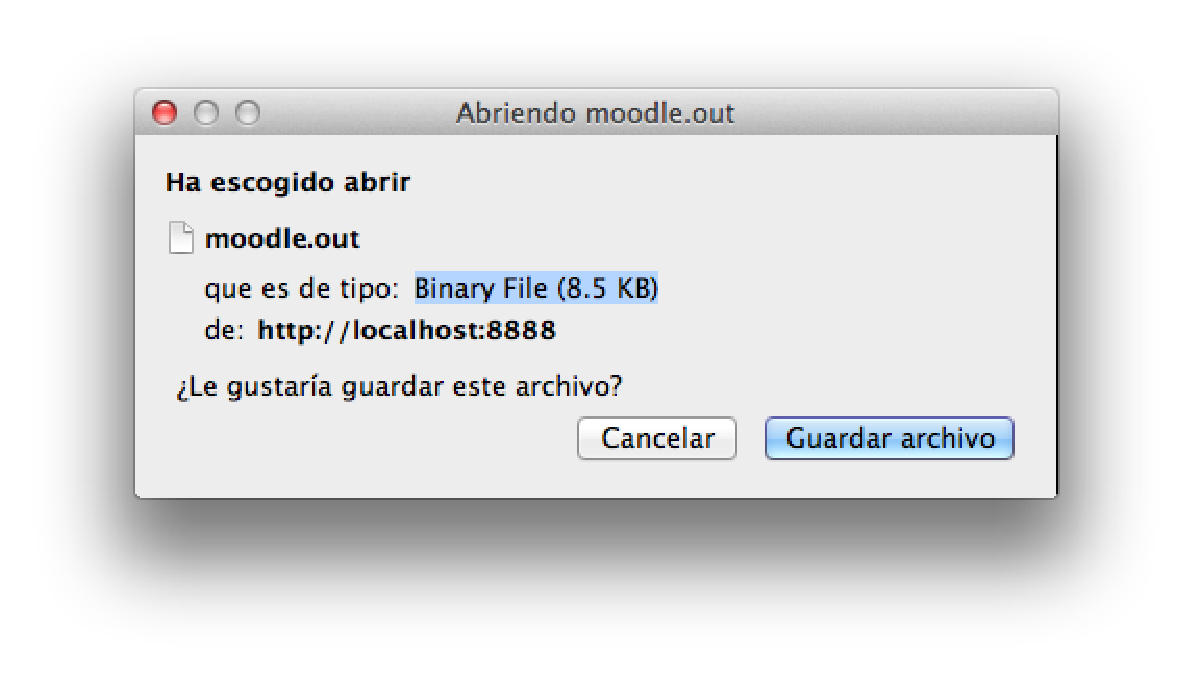
\includegraphics[scale=0.40]{./img/ecompile.eps}
	\caption{Editor de código. Descarga de ejecutable en Mac OS.}
	\end{center}
\end{figure}
















	